%\VignetteIndexEntry{Lexis functions for representation and analysis of follow-up data}

\documentclass[a4paper, dvipsnames, twoside, 12pt]{report}
\newcommand{\Title}{\texttt{Lexis} functions in \texttt{Epi}\\
  for representation and analysis of\\ follow-up data}
\newcommand{\Tit}{\texttt{Lexis} FU}
\newcommand{\Version}{Version 11}
\newcommand{\Dates}{November 2024}
\newcommand{\Where}{SDCC}
\newcommand{\Homepage}{\url{http://bendixcarstensen.com/} }
\newcommand{\Faculty}{\begin{tabular}{rl}
Bendix Carstensen
  & Steno Diabetes Center Copenhagen, Herlev, Denmark\\
  & {\small \& Department of Biostatistics,
               University of Copenhagen} \\
  & \texttt{b@bxc.dk} \quad \texttt{bcar0029@regionh.dk} \\
  & \url{http://BendixCarstensen.com} \\[1em]
                      \end{tabular}}

%----------------------------------------------------------------------
% Packages
%\usepackage[inline]{showlabels}
%\usepackage[latin1]{inputenc}
\usepackage[utf8]{inputenc}
\usepackage[T1]{fontenc}
\usepackage[english]{babel}
\usepackage[font=it,labelfont=normalfont]{caption}
\usepackage[colorlinks,urlcolor=blue,linkcolor=red,citecolor=Maroon]{hyperref}
\usepackage[dvipsnames]{xcolor}
\usepackage[super]{nth}
% \usepackage[retainorgcmds]{IEEEtrantools}
\usepackage[noae]{Sweave}
\usepackage[ae,hyper]{Rd}
% \usepackage[noae]{C:/util/R/R-4.2.0/share/texmf/tex/latex/Sweave}
% \usepackage{C:/util/R/R-4.2.0/share/texmf/tex/latex/Rd}
\usepackage{makeidx,floatflt,amsmath,amsfonts,amsbsy,enumitem,dcolumn,needspace}
\usepackage{ifthen,calc,eso-pic,everyshi}
\usepackage{booktabs,longtable,rotating,graphicx,subfig}
\usepackage{pdfpages,verbatim,fancyhdr,datetime,afterpage}
\usepackage[abspath]{currfile}
% \usepackage{times}
\renewcommand{\textfraction}{0.0}
\renewcommand{\topfraction}{1.0}
\renewcommand{\bottomfraction}{1.0}
\renewcommand{\floatpagefraction}{0.9}
\definecolor{blaa}{RGB}{99,99,255}
\DeclareGraphicsExtensions{.png,.pdf,.jpg}
% Make the Sweave output nicer (slightly mor compact)
\DefineVerbatimEnvironment{Sinput}{Verbatim}{fontsize=\small,fontshape=sl,formatcom=\color{BlueViolet}}
\DefineVerbatimEnvironment{Soutput}{Verbatim}{fontsize=\small,formatcom=\color{Sepia},xleftmargin=0em}
\DefineVerbatimEnvironment{Scode}{Verbatim}{fontsize=\small}
\fvset{listparameters={\setlength{\topsep}{-0.1ex}}}
\renewenvironment{Schunk}%
{\renewcommand{\baselinestretch}{0.87} \vspace{\topsep}}%
{\renewcommand{\baselinestretch}{1.00} \vspace{\topsep}}
% \renewenvironment{knitrout}
% {\renewcommand{\baselinestretch}{0.87}}
% {\renewcommand{\baselinestretch}{1.00}}
% This is a file of useful extra commands snatched from
% Michael Hills, David Clayton, Bendix Carstensen & Esa Laara.
%

% Commands to draw observation lines on follow-up diagrams
%
% Horizontal lines
%
\providecommand{\hfail}[1]{\begin{picture}(250,5)
      \put(0,0){\line(1,0){#1}}
      \put(#1,0){\circle*{5}}
   \end{picture}}

\providecommand{\hcens}[1]{\begin{picture}(250,5)
      \put(0,0){\line(1,0){#1}}
      \put(#1,0){\line(0,1){2.5}}
      \put(#1,0){\line(0,-1){2.5}}
   \end{picture}}

%
% Diagonals for Lexis diagrams
%
\providecommand{\dfail}[1]{\begin{picture}(250,250)
      \put(0,0){\line(1,1){#1}}
      \put(#1,#1){\circle*{5}}
   \end{picture}}

\providecommand{\dcens}[1]{\begin{picture}(250,250)
      \put(0,0){\line(1,1){#1}}
%      \put(#1,#1){\line(0,1){2.5}}
%      \put(#1,#1){\line(0,-1){2.5}}
% BxC Changed this to an open circle instead of a line
      \put(#1,#1){\circle{5}}
   \end{picture}}

%
% Horizontal range diagrams
%
\providecommand{\hrange}[1]{\begin{picture}(200,5)
     \put(0,0){\circle*{5}}
     \put(0,0){\line(1,0){#1}}
     \put(0,0){\line(-1,0){#1}}
   \end{picture}}

%
% Tree drawing
%
\providecommand{\Tree}[3]{\setlength{\unitlength}{#1\unitlength}\begin{picture}(0,0)
   \put(0,0){\line(3, 2){1}}
   \put(0,0){\line(3,-2){1}}
   \put(0.81, 0.54){\makebox(0,0)[br]{\footnotesize #2\ }}
   \put(0.81,-0.54){\makebox(0,0)[tr]{\footnotesize #3\ }}
\end{picture}}

\providecommand{\Wtree}[3]{\setlength{\unitlength}{#1\unitlength}\begin{picture}(0,0)
   \put(0,0){\line(1, 1){1}}
   \put(0,0){\line(1,-1){1}}
   \put(0.8,0.8){\makebox(0,0)[br]{\footnotesize #2\ }}
   \put(0.8,-0.8){\makebox(0,0)[tr]{\footnotesize #3\ }}
\end{picture}}

\providecommand{\Ntree}[3]{\setlength{\unitlength}{#1\unitlength}\begin{picture}(0,0)
   \put(0,0){\line(2, 1){1}}
   \put(0,0){\line(2,-1){1}}
   \put(0.8,0.4){\makebox(0,0)[br]{\footnotesize #2\ }}
   \put(0.8,-0.4){\makebox(0,0)[tr]{\footnotesize #3\ }}
\end{picture}}

\providecommand{\Nutree}[3]{\setlength{\unitlength}{#1\unitlength}\begin{picture}(0,0)
   \put(0,0){\line(2, 1){#1}}
   \put(0,0){\line(2,-1){#1}}
   \put(0.8,0.4){\makebox(0,0)[br]{#2\ }}
   \put(0.8,-0.4){\makebox(0,0)[tr]{#3\ }}
\end{picture}}

%
% Tree drawing
%
\providecommand{\tree}[3]{\setlength{\unitlength}{#1}\begin{picture}(0,0)
   \put(0,0){\line(3,2){1}}
   \put(0,0){\line(3,-2){1}}
   \put(0.81,0.54){\makebox(0,0)[br]{\footnotesize #2\ }}
   \put(0.81,-0.54){\makebox(0,0)[tr]{\footnotesize #3\ }}
\end{picture}}

\providecommand{\wtree}[3]{\setlength{\unitlength}{#1}\begin{picture}(0,0)
   \put(0,0){\line(1,1){1}}
   \put(0,0){\line(1,-1){1}}
   \put(0.8,0.8){\makebox(0,0)[br]{\footnotesize #2\ }}
   \put(0.8,-0.8){\makebox(0,0)[tr]{\footnotesize #3\ }}
\end{picture}}

\providecommand{\ntree}[3]{\setlength{\unitlength}{#1}\begin{picture}(0,0)
   \put(0,0){\line(2,1){1}}
   \put(0,0){\line(2,-1){1}}
   \put(0.8,0.4){\makebox(0,0)[br]{\footnotesize #2\ }}
   \put(0.8,-0.4){\makebox(0,0)[tr]{\footnotesize #3\ }}
\end{picture}}

\providecommand{\nutree}[3]{\begin{picture}(0,0)
   \put(0,0){\line(2,1){#1}}
   \put(0,0){\line(2,-1){#1}}
   \put(0.8,0.4){\makebox(0,0)[br]{#2\ }}
   \put(0.8,-0.4){\makebox(0,0)[tr]{#3\ }}
\end{picture}}

%
% Other commands
%
\providecommand{\ip}[2]{\langle #1 \vert #2 \rangle} 
\providecommand{\I}{\text{\rm gI}}
\providecommand{\prob}[0]{\text{\rm Pr}}
\providecommand{\nhy}[0]{_{\oslash}}
\providecommand{\true}[0]{_{\text{\rm \tiny T}}}
\providecommand{\hyp}[0]{_{\text{\rm \tiny H}}}
% \providecommand{\mpydiv}[0]{\stackrel{\textstyle \times}{\div}}
% Changed to slightly smaller symbols
\providecommand{\mpydiv}[0]{\stackrel{\scriptstyle\times}{\scriptstyle\div}}
\providecommand{\mie}[1]{{\it #1}}
\providecommand{\mycircle}[0]{\circle*{5}}
\providecommand{\smcircle}[0]{\circle*{1}}
\providecommand{\corner}[0]{_{\text{\rm \tiny C}}}
\providecommand{\ind}[0]{\hspace{10pt}}
\providecommand{\gap}[0]{\\[5pt]}
\renewcommand{\S}[0]{section~}
\providecommand{\blank}[0]{$\;\,$}
\providecommand{\vone}{\vspace{1cm}}
\providecommand{\ljust}[1]{\multicolumn{1}{l}{#1}}
\providecommand{\cjust}[1]{\multicolumn{1}{c}{#1}}
\providecommand{\transpose}{^{\text{\sf T}}}
\providecommand{\histog}[5]{\rule{1mm}{#1mm}\,\rule{1mm}{#2mm}\,\rule{1mm}{#3mm}\,\rule{1mm}{#4mm}\,\rule{1mm}{#5mm}}
\providecommand{\pmiss}{P_{\mbox{\tiny miss}}}

% Below is BxCs commands inserted

% Only works with hyperref package:
\newcommand{\mailto}[1]{\href{mailto:#1}{\tt #1}}

\providecommand{\bc}{\begin{center}}
\providecommand{\ec}{\end{center}}
\providecommand{\bd}{\begin{description}}
\providecommand{\ed}{\end{description}}
\providecommand{\bi}{\begin{itemize}}
\providecommand{\ei}{\end{itemize}}
\providecommand{\bn}{\begin{equation}}
\providecommand{\en}{\end{equation}}
\providecommand{\be}{\begin{enumerate}}
\providecommand{\ee}{\end{enumerate}}
\providecommand{\bes}{\begin{eqnarray*}}
\providecommand{\ees}{\end{eqnarray*}}

\DeclareMathOperator{\Pp}{P}
\DeclareMathOperator{\pp}{p}
% \providecommand{\p}{{\mathrm p}}
\providecommand{\e}{{\mathrm e}}
\providecommand{\D}{{\mathrm D}}
\providecommand{\dif}{{\,\mathrm d}}
\providecommand{\pmat}[1]{\Pp\!\left\{#1\right\}}
\providecommand{\ptxt}[1]{\Pp\!\left\{\text{#1}\right\}}
\providecommand{\E}{\text{\rm E}}
\providecommand{\V}{\text{\rm V}}
\providecommand{\BLUP}{\text{\rm BLUP}}
\providecommand{\se}{\text{\rm s.e.}}
\providecommand{\sem}{\text{\rm s.e.m.}}
\providecommand{\std}{\text{\rm std}}
\providecommand{\sd}{\text{\rm s.d.}}
\providecommand{\Var}{\text{\rm var}}
\providecommand{\VAR}{\text{\rm var}}
\providecommand{\var}{\text{\rm var}}
\providecommand{\cov}{\text{\rm cov}}
\providecommand{\corr}{\text{\rm corr}}
\providecommand{\mean}{\text{\rm mean}}
\providecommand{\CV}{\text{\rm CV}}
\providecommand{\median}{\text{\rm median}}
\providecommand{\cv}{\text{\rm c.v.}}
\providecommand{\erf}{\text{\rm erf}}
\providecommand{\ef}{\text{\rm ef}}
\providecommand{\SSD}{\text{\rm SSD}}
\providecommand{\SPD}{\text{\rm SPD}}
\providecommand{\odds}{\text{\rm odds}}
\providecommand{\bin}{\text{\rm binom}}
\providecommand{\half}{\frac{1}{2}}
% \providecommand{\td}[0]{\stackrel{\textstyle \times}{\div}}
% Changed to slightly smaller symbols
\providecommand{\td}[0]{\stackrel{\scriptstyle \times}{\scriptstyle \div}}
\providecommand{\dt}[0]{\stackrel{\scriptstyle \div}{\scriptstyle \times}}
\providecommand{\diag}{\text{\rm diag}}
\providecommand{\det}{\text{\rm det}}
\providecommand{\dim}{\text{\rm dim}}
\providecommand{\spcol}{\text{\rm span}}
\providecommand{\logit}{\text{\rm logit}}
% \providecommand{\link}{\text{\rm link}}
\providecommand{\spn}{\text{\rm span}}
\providecommand{\CI}{\text{\rm CI}}
\providecommand{\IP}{\text{\rm IP}}
\providecommand{\OR}{\text{\rm OR}}
\providecommand{\RR}{\text{\rm RR}}
\providecommand{\ER}{\text{\rm ER}}
\providecommand{\EM}{\text{\rm EM}}
\providecommand{\EF}{\text{\rm EF}}
\providecommand{\RD}{\text{\rm RD}}
\providecommand{\AC}{\text{\rm AC}}
\providecommand{\AF}{\text{\rm AF}}
\providecommand{\PAF}{\text{\rm PAF}}
\providecommand{\AR}{\text{\rm AR}}
\providecommand{\CR}{\text{\rm CR}}
\providecommand{\PAR}{\text{\rm PAR}}
\providecommand{\EL}{\text{\rm EL}}
\providecommand{\ERL}{\text{\rm ERL}}
\providecommand{\YLL}{\text{\rm YLL}}
\providecommand{\SD}{\text{\rm SD}}
\providecommand{\SE}{\text{\rm SE}}
\providecommand{\SEM}{\text{\rm SEM}}
\providecommand{\SR}{\text{\rm SR}}
\providecommand{\SMR}{\text{\rm SMR}}
\providecommand{\RSR}{\text{\rm RSR}}
\providecommand{\CMF}{\text{\rm CMF}}
\providecommand{\pvp}{\text{\rm PV$+$}}
\providecommand{\pvn}{\text{\rm PV$-$}}
\providecommand{\R}{{\textsf{\textbf{R}}}}
\providecommand{\sas}{\textsl{\textbf{SAS}}}
\providecommand{\SAS}{\textsl{\textbf{SAS}}}
%\providecommand{\gap}[0]{\\[5pt]}
%\providecommand{\blank}[0]{$\;\,$}
% Conditional independence sign from Philip Dawid
\providecommand{\cip}{\mbox{$\perp\!\!\!\perp$}}

%%% Commands to comment out parts of the text
\providecommand{\GLEM}[1]{}
\providecommand{\FORGETIT}[1]{}
\providecommand{\OMIT}[1]{}

%%% Insert output from program in small text
%%% (requires package verbatim)
\providecommand{\insoutsmall}[1]{
% \small
 \footnotesize
 \renewcommand{\baselinestretch}{0.8}
 \verbatiminput{#1}
 \renewcommand{\baselinestretch}{1.0}
 \normalsize
}
\providecommand{\insout}[1]{
 \scriptsize
 \renewcommand{\baselinestretch}{0.8}
 \verbatiminput{#1}
 \renewcommand{\baselinestretch}{1.0}
 \normalsize
}
\providecommand{\insouttiny}[1]{
\tiny
\renewcommand{\baselinestretch}{0.8}
\verbatiminput{#1}
\renewcommand{\baselinestretch}{1.0}
\normalsize
}

% From Esa:
\providecommand{\T}{\text{\rm \small{T}}}
\providecommand{\id}{\text{\rm id}}
\providecommand{\Dev}{\text{\rm Dev}}
\providecommand{\Bin}{\text{\rm Bin}}
\providecommand{\probit}{\text{\rm probit}}
\providecommand{\cloglog}{\text{\rm cloglog}}

% Special commands to include output from R, Bugs and Stata

\providecommand{\Rin}[2]{
\subsection{\texttt{#1.R}}
#2

\insout{./R/#1.Rout}

}

\providecommand{\Statain}[2]{
\subsection{\texttt{#1.do}}
#2

\insout{./do/#1.log}

}

\providecommand{\Bugsin}[2]{
\subsection{\texttt{#1.bug}}
#2

\insout{./bugs/#1.bug}

}

\newlength{\wdth}
\providecommand{\fxbl}[1]{\settowidth{\wdth}{#1} \makebox[\wdth]{}}

%%% Local Variables:
%%% mode: latex
%%% TeX-master: t
%%% End:


%----------------------------------------------------------------------
% Set up layout of pages
\oddsidemargin 1mm
\evensidemargin 1mm
\topmargin -10mm
\headheight 8mm
\headsep 5mm
\textheight 240mm
\textwidth 165mm
%\footheight 5mm
\footskip 15mm
\renewcommand{\topfraction}{0.9}
\renewcommand{\bottomfraction}{0.9}
\renewcommand{\textfraction}{0.1}
\renewcommand{\floatpagefraction}{0.9}
\renewcommand{\headrulewidth}{0.1pt}
\setcounter{secnumdepth}{2}
\setcounter{tocdepth}{3}

%----------------------------------------------------------------------
% How to insert a figure in a .rnw file
\newcommand{\rwpre}{./graph/gr}
\newcommand{\insfig}[3]{
\begin{figure}[h]
  \centering
  \includegraphics[width=#2\textwidth]{\rwpre-#1}
% \caption{#3}
  \caption{#3\hfill\mbox{\footnotesize \textrm{\tt \rwpre-#1}}}
  \label{fig:#1}
% \afterpage{\clearpage}
\end{figure}}
\newcommand{\linput}[1]{
% \clearpage 
\afterpage{\hfill \ldots now input from \texttt{#1.tex}\\} 
\fancyfoot[OR,EL]{\footnotesize \texttt{#1.tex}} 
\input{#1}}

%----------------------------------------------------------------------
% Here is the document starting with the titlepage
\begin{document}

%----------------------------------------------------------------------
% The title page
\setcounter{page}{1}
\pagenumbering{roman}
\pagestyle{plain}
\thispagestyle{empty}
% \vspace*{0.05\textheight}
\flushright
% The blank below here is necessary in order not to muck up the
% linespacing in title if it has more than 2 lines
{\Huge \bfseries \Title

}\ \\[-1.5ex]
\noindent\textcolor{blaa}{\rule[-1ex]{\textwidth}{5pt}}\\[2.5ex]
\large
\Where \\
\Dates \\
\Homepage \\
\Version \\[1em]
\normalsize
Compiled \today,\ \currenttime\\
from: \texttt{\currfileabspath}\\[1em]
% \input{wordcount}
\normalsize
\vfill
\Faculty
% End of titlepage
\newpage

%----------------------------------------------------------------------
% Table of contents
\tableofcontents
% \listoftables
% \listoffigures
\clearpage
% \begingroup
% \let\clearpage\relax
% \listoftables
% \listoffigures
% \endgroup

%----------------------------------------------------------------------
% General text layout
\raggedright
\parindent 1em
\parskip 0ex
\cleardoublepage

%----------------------------------------------------------------------
% General page style
\pagenumbering{arabic}
\setcounter{page}{1}
\pagestyle{fancy}
\renewcommand{\chaptermark}[1]{\markboth{\textsl{#1}}{}}
\renewcommand{\sectionmark}[1]{\markright{\thesection\ \textsl{#1}}{}}
\fancyhead[EL]{\bf \thepage \quad \rm \rightmark}
\fancyhead[ER]{\rm \Tit}
\fancyhead[OL]{\rm \leftmark}
\fancyhead[OR]{\rm \rightmark \quad \bf \thepage}
\fancyfoot{}

\renewcommand{\rwpre}{./01flup}

\chapter*{Introduction}
\addcontentsline{toc}{chapter}{Introduction}

\section{Technicalities}
First we set some graphics parameters for convenience and load the
packages needed:
\begin{Schunk}
\begin{Sinput}
> options(width = 90,
+         show.signif.stars = FALSE,
+         SweaveHooks=list(fig = function()
+                          par(mar = c(3, 3, 1, 1),
+                              mgp = c(3, 1, 0) / 1.6,
+                              las = 1,
+                             lend = "butt",
+                              bty = "n")))
> library(Epi)
> library(popEpi)
> library(survival)
> clear()
\end{Sinput}
\end{Schunk}
% must be after clear() because 'anfang' is used at the end
\begin{Schunk}
\begin{Soutput}
     R   Epi   popEpi
 4.5.0  2.60   0.4.13
\end{Soutput}
\end{Schunk}

\section{About this vignette}

This vignette is an introduction to (parts of) the \texttt{Lexis}
machinery in the \texttt{Epi} package, intended for representation and
manipulation of follow-up data (``event history data'') from studies
where exact dates of events (state transitions) are known. It
accommodates follow-up through multiple states and on multiple time
scales.

We use a data example from the \texttt{Epi} package to illustrate the
set-up of a simple \texttt{Lexis} object (a data frame of follow-up
intervals), as well as the subdivision of follow-up intervals needed
for multistate representation and analysis of transition rates by
flexible parametric functions.

The first chapter is exclusively on manipulation of the follow-up
representation, but it points to the subsequent chapter where analysis
is based on a \texttt{Lexis} representation with very small follow-up
intervals.

Chapter 2 uses analysis of mortality rates among Danish diabetes
patients (available in the \texttt{Epi} package) currently on insulin
treatment or not, to illustrate the use of \texttt{Lexis} object in
the analysis of rates.

Chapter 3 discuss the use of multiple time scales,
chapter 4 discusses creation and manipulation of multistate data, and
chapter 5 is a list of all \texttt{Lexis} functions.

\section{History}

The \texttt{Lexis} machinery in the \texttt{Epi} package was first
conceived and implemented by Martyn
Plummer\cite{Plummer.2011,Carstensen.2011a}, and since its first
appearance in the \texttt{Epi} package in 2008 it has been expanded
with a number of utilities. An overview of these can be found in the
last chapter of this note, \hyperlink{lexfun}{``\texttt{Lexis}
  functions''}.

\subsection{Wilhelm Lexis}

\begin{minipage}[t]{0.6\linewidth}
  \raggedright
  The \code{Lexis} machinery is named after the German demographer
  and economist Wilhelm Lexis (full name Wilhelm Hector Richard
  Albrecht Lexis, 17 July 1837 -- 24 August 1914), who in his book
  ``Einleitung in die Theorie der Bev\"{o}lkerungsstatistik''
  (Introduction to the theory of population statistics, Strassburg,
  1875), devised a diagram showing follow-up of persons on two time
  scales, notably calendar time and age. The diagram that nowadays is
  called a Lexis diagram, is usually drawn in a slightly different
  manner than that Lexis used in his book.

  \quad The display of follow-up on two timescales naturally leads to
  representation on several time scales and statistical modeling of
  occurrence rates with two (or more) timescales as explanatory
  terms. Hence the naming of the machinery after Wilhelm Lexis.
\end{minipage}
\hfill
\begin{minipage}[t]{0.35\linewidth}
  \ \\[-1em]
  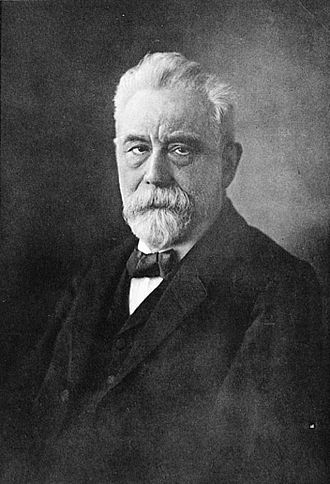
\includegraphics[width=1.0\textwidth]{Wilhelm_Lexis}
\end{minipage}

\subsection{Modeling of rates}

In 1976, Theodore R. Holford published a paper: ``Life Tables with
Concomitant Information'', \cite{Holford.1976} where he detailed
estimation in models for occurrence rates based on subdivision of
follow-up time in smaller intervals, including the handling of
time-dependent variables.  In 1980 John Whitehead published a paper:
``Fitting Cox's regression model to survival data using GLIM'',
\cite{Whitehead.1980} in which he devised the likelihood of a model
for many small time bands with constant intensity in each, and
demonstrated that Cox's partial likelihood could be seen as a Poisson
likelihood. It is essentially these two papers that underlie the
time-splitting and subsequent modeling of transition
rates in this vignette.\\[1em]
\noindent
\ldots so there is very little (if anything) new in this note.

\chapter{Representation of follow-up data in \texttt{Epi}}

In the \texttt{Epi}-package, follow-up data is represented by adding
some extra variables and a few attributes to a data frame. Such a data
frame is called a \texttt{Lexis} object. The tools for handling
follow-up data then use the structure of this for special plots,
tabulations and modeling.

Specifically, follow-up data requires a choice of time scale, a time
of entry, a time of exit and an indication of the status at exit
(normally either ``alive'' or ``dead'') for each person. Implicitly is
also assumed a status \emph{during} the follow-up (usually ``alive'').

\begin{figure}[htbp]
  \centering
\setlength{\unitlength}{1pt}
\begin{picture}(210, 70)(0, 75)
%\scriptsize
\thicklines
 \put(  0, 80){\makebox(0, 0)[r]{Age-scale}}
 \put( 50, 80){\line(1, 0){150}}
 \put( 50, 80){\line(0, 1){5}}
 \put(100, 80){\line(0, 1){5}}
 \put(150, 80){\line(0, 1){5}}
 \put(200, 80){\line(0, 1){5}}
 \put( 50, 77){\makebox(0, 0)[t]{35}}
 \put(100, 77){\makebox(0, 0)[t]{40}}
 \put(150, 77){\makebox(0, 0)[t]{45}}
 \put(200, 77){\makebox(0, 0)[t]{50}}

 \put(  0, 115){\makebox(0, 0)[r]{Follow-up}}

 \put( 80, 105){\makebox(0, 0)[r]{\small Two}}
 \put( 90, 105){\line(1, 0){87}}
 \put( 90, 100){\line(0, 1){10}}
 \put(100, 100){\line(0, 1){10}}
 \put(150, 100){\line(0, 1){10}}
 \put(180, 105){\circle{6}}
 \put( 95, 110){\makebox(0, 0)[b]{1}}
 \put(125, 110){\makebox(0, 0)[b]{5}}
 \put(165, 110){\makebox(0, 0)[b]{3}}

 \put( 50, 130){\makebox(0, 0)[r]{\small One}}
 \put( 60, 130){\line(1, 0){70}}
 \put( 60, 125){\line(0, 1){10}}
 \put(100, 125){\line(0, 1){10}}
 \put(130, 130){\circle*{6}}
 \put( 80, 135){\makebox(0, 0)[b]{4}}
 \put(115, 135){\makebox(0, 0)[b]{3}}
\end{picture}
  \caption{\it Follow-up of two persons on the age-scale}
  \label{fig:fu2}
\end{figure}

\section{Time scales}

A time scale is a variable that varies deterministically \emph{within}
each person during follow-up, \textit{e.g.}:
\begin{itemize}[noitemsep]
  \item Age
  \item Calendar time
  \item Time since start of treatment
  \item Time since relapse
  \end{itemize}
All time scales advance at the same pace, so the time followed is the
same on all time scales. Therefore, it will suffice to use only the
entry point on each of the time scales, for example:
\begin{itemize}[noitemsep]
  \item Age at entry
  \item Date of entry
  \item Time at treatment---\emph{at} treatment, time since treatment
    is 0, but persons may enter before or after treatment beginnng.
  \item Time at relapse---\emph{at} relapse, time since relapse
    is 0, but persons may enter before or after relapse.
\end{itemize}
In the \texttt{Epi} package, follow-up in a cohort is represented in a
\texttt{Lexis} object. A \texttt{Lexis} object is a data frame with
some extra structure to represent the follow-up. For the
\texttt{DMlate} dataset of follow-up of diabetes patients in Denmark---
with recorded date of birth, date of diabetes, date of first insulin use,
date of first oral drug use, date of exit and date of death---we can
construct a \texttt{Lexis} object by first including follow-up from
entry at date of diabetes (\texttt{dodm}) to exit (\texttt{dox}).
The dates should \emph{not} be in \texttt{Date} format; some data
manipulations in \texttt{Lexis} will crash if they are.
\begin{Schunk}
\begin{Sinput}
> data(DMlate)
> head(DMlate)
\end{Sinput}
\begin{Soutput}
       sex    dobth     dodm    dodth    dooad doins      dox
50185    F 1940.256 1998.917       NA       NA    NA 2009.997
307563   M 1939.218 2003.309       NA 2007.446    NA 2009.997
294104   F 1918.301 2004.552       NA       NA    NA 2009.997
336439   F 1965.225 2009.261       NA       NA    NA 2009.997
245651   M 1932.877 2008.653       NA       NA    NA 2009.997
216824   F 1927.870 2007.886 2009.923       NA    NA 2009.923
\end{Soutput}
\begin{Sinput}
> dmL <- Lexis(entry = list(per = dodm,
+                           age = dodm-dobth,
+                           tfD = 0),
+               exit = list(per = dox),
+        exit.status = factor(!is.na(dodth),
+                             labels = c("DM", "Dead")),
+               data = DMlate)
\end{Sinput}
\begin{Soutput}
NOTE: entry.status has been set to "DM" for all.
NOTE: Dropping  4  rows with duration of follow up < tol
\end{Soutput}
\begin{Sinput}
> timeScales(dmL)
\end{Sinput}
\begin{Soutput}
[1] "per" "age" "tfD"
\end{Soutput}
\end{Schunk}
The 4 excluded persons are persons with date of diabetes equal to date
of death.

The \texttt{entry} argument is a \emph{named} list with the entry
points on each of the time scales we want to use. The names of the
list defines the names of the time scales. The \texttt{exit} argument
gives the exit time on \emph{one} of the time scales, so the name of
the element in this list must match one of the names of the
\texttt{entry} list. This is sufficient, because the follow-up time on
all time scales is the same, in this case
$\mathtt{dox}-\mathtt{dodm}$.

The \texttt{exit.status} will normally be a categorical variable (a
\emph{factor}) that indicates the exit status --- in this case whether
the person (still) is in state \texttt{DM} or exits to \texttt{Dead}
at the end of follow-up. We could also specify an
\texttt{entry.status}; the default is to assume that all persons enter
in the \emph{first} level of the factor \texttt{exit.state}s --- in
this case \texttt{DM} (because $\mathtt{FALSE}<\mathtt{TRUE}$).

Now take a look at the result:
\begin{Schunk}
\begin{Sinput}
> str(dmL)
\end{Sinput}
\begin{Soutput}
Classes 'Lexis' and 'data.frame':	9996 obs. of  14 variables:
 $ per    : num  1999 2003 2005 2009 2009 ...
 $ age    : num  58.7 64.1 86.3 44 75.8 ...
 $ tfD    : num  0 0 0 0 0 0 0 0 0 0 ...
 $ lex.dur: num  11.08 6.689 5.446 0.736 1.344 ...
 $ lex.Cst: Factor w/ 2 levels "DM","Dead": 1 1 1 1 1 1 1 1 1 1 ...
 $ lex.Xst: Factor w/ 2 levels "DM","Dead": 1 1 1 1 1 2 1 1 2 1 ...
 $ lex.id : int  1 2 3 4 5 6 7 8 9 10 ...
 $ sex    : Factor w/ 2 levels "M","F": 2 1 2 2 1 2 1 1 2 1 ...
 $ dobth  : num  1940 1939 1918 1965 1933 ...
 $ dodm   : num  1999 2003 2005 2009 2009 ...
 $ dodth  : num  NA NA NA NA NA ...
 $ dooad  : num  NA 2007 NA NA NA ...
 $ doins  : num  NA NA NA NA NA NA NA NA NA NA ...
 $ dox    : num  2010 2010 2010 2010 2010 ...
 - attr(*, "time.scales")= chr [1:3] "per" "age" "tfD"
 - attr(*, "time.since")= chr [1:3] "" "" ""
 - attr(*, "breaks")=List of 3
  ..$ per: NULL
  ..$ age: NULL
  ..$ tfD: NULL
\end{Soutput}
\begin{Sinput}
> head(dmL)[, 1:11]
\end{Sinput}
\begin{Soutput}
 lex.id     per   age tfD lex.dur lex.Cst lex.Xst sex   dobth    dodm   dodth
      1 1998.92 58.66   0   11.08      DM      DM   F 1940.26 1998.92      NA
      2 2003.31 64.09   0    6.69      DM      DM   M 1939.22 2003.31      NA
      3 2004.55 86.25   0    5.45      DM      DM   F 1918.30 2004.55      NA
      4 2009.26 44.04   0    0.74      DM      DM   F 1965.23 2009.26      NA
      5 2008.65 75.78   0    1.34      DM      DM   M 1932.88 2008.65      NA
      6 2007.89 80.02   0    2.04      DM    Dead   F 1927.87 2007.89 2009.92
\end{Soutput}
\end{Schunk}
The \texttt{Lexis} object \texttt{dmL} has a variable for each time
scale, the value of which is the entry time for each person on this time
scale. The length of the follow-up time is in the variable
\texttt{lex.dur} (\texttt{dur}ation).  Note that the exit status is in
the variable \texttt{lex.Xst} (e\texttt{X}it \texttt{st}ate). The
variable \texttt{lex.Cst} indicates the state where follow-up takes
place (\texttt{C}urrent \texttt{st}ate), in this case \texttt{DM}
(alive with diabetes) for all persons. This implies that observations
\emph{censored} in state \texttt{A}, say, are characterized by
having $\mathtt{lex.Cst} = \mathtt{lex.Xst} = \mathtt{A}$.

There is a \texttt{summary} function for \texttt{Lexis} objects that
lists the number of transitions and records as well as the total
amount of follow-up time; it also (optionally) prints information
about the names of the variables that constitute the time scales:
\begin{Schunk}
\begin{Sinput}
> summary(dmL, timeScales = TRUE)
\end{Sinput}
\begin{Soutput}
Transitions:
     To
From   DM Dead  Records:  Events: Risk time:  Persons:
  DM 7497 2499      9996     2499   54273.27      9996

Timescales:
per age tfD 
 ""  ""  "" 
\end{Soutput}
\end{Schunk}
It is possible to get a visualization of the follow-up along the
time scales chosen by using the \texttt{plot} method for \texttt{Lexis}
objects. \texttt{dmL} is an object of \emph{class} \texttt{Lexis}, so
using the function \texttt{plot()} on it means that \R\ will look for
the function \texttt{plot.Lexis} and use this function.
\begin{Schunk}
\begin{Sinput}
> plot(dmL)
\end{Sinput}
\end{Schunk}
The function allows quite a bit of control over the output, and a
\texttt{points.Lexis} function allows plotting of the endpoints of
follow-up:
\begin{Schunk}
\begin{Sinput}
> par(mar = c(3, 3, 1, 1), mgp = c(3, 1, 0) / 1.6)
> plot(dmL, 1:2, lwd = 1, col = c("blue", "red")[dmL$sex],
+      grid = TRUE, lty.grid = 1, col.grid = gray(0.7),
+      xlim = 1960 + c(0, 60), xaxs = "i",
+      ylim =   40 + c(0, 60), yaxs = "i", las = 1)
> points(dmL, 1:2, pch = c(NA, 3)[dmL$lex.Xst],
+        col = "lightgray", lwd = 3, cex = 0.3)
> points(dmL, 1:2, pch = c(NA, 3)[dmL$lex.Xst],
+        col = c("blue", "red")[dmL$sex], lwd = 1, cex = 0.3)
> box(bty = 'o')
\end{Sinput}
\end{Schunk}
In the above code you will note that the values of the arguments
\texttt{col} and \texttt{pch} are indexed by factors, using the
convention in \R\ that the index is taken as \emph{number of the
  level} of the supplied factor. Thus \texttt{c("blue",
  "red")[dmL\$sex]} is \texttt{"blue"} when \texttt{sex} is \texttt{M}
(the first level of \texttt{sex}) and.  \texttt{"red"} when
\texttt{sex} is \texttt{F} (the second level of \texttt{sex}).

The results of these two plotting commands are in figure
\ref{fig:Lexis-diagram}, p. \pageref{fig:Lexis-diagram}.
\begin{figure}[tb]
\centering
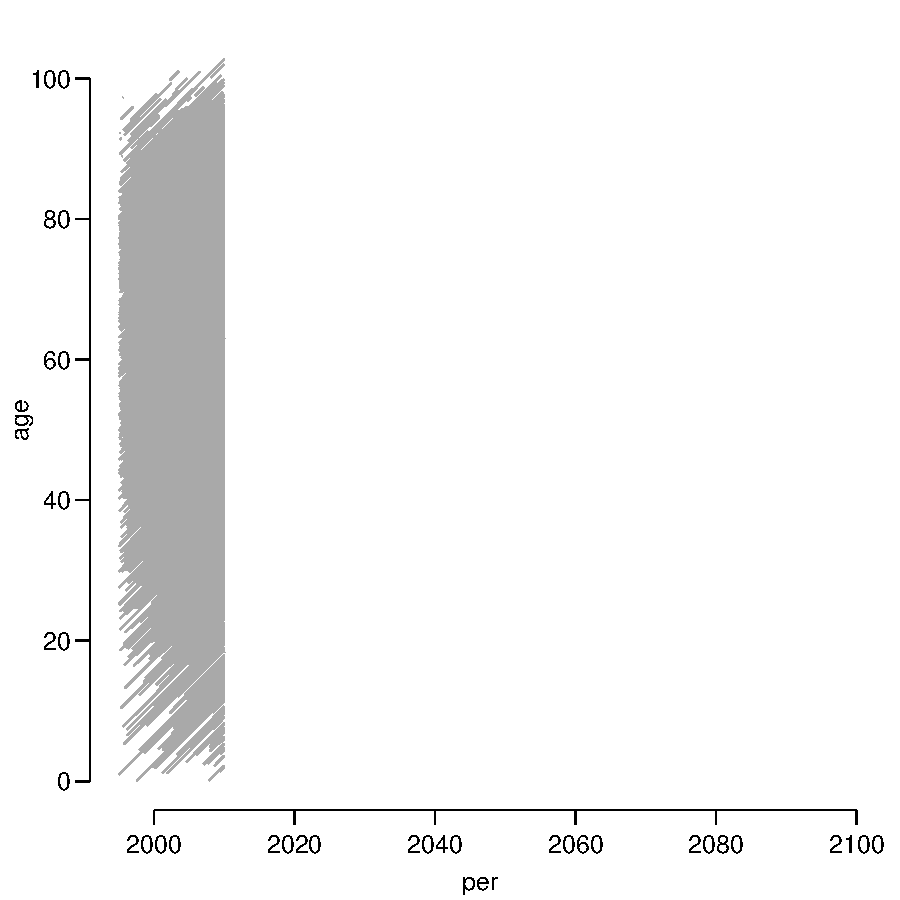
\includegraphics[width = 0.35\textwidth]{01flup-dmL1}
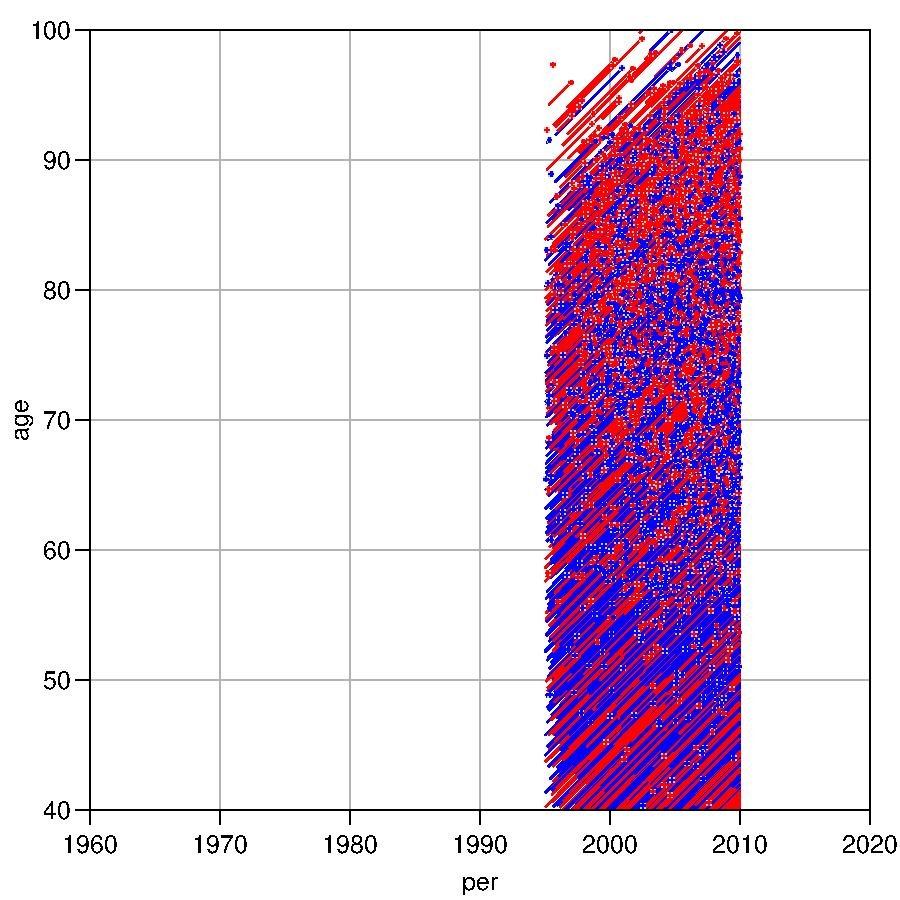
\includegraphics[width = 0.63\textwidth]{01flup-dmL2}
\caption{\it Lexis diagram of the \textrm{\tt DMlate} dataset; left
  panel is the default version, right panel is with some bells and
  whistles. The red lines are for women, blue for men, crosses
  indicate deaths.}
\label{fig:Lexis-diagram}
\end{figure}

\section{Splitting the follow-up time along a time scale}

In next chapter we shall conduct statistical analysis of mortality
rates, and a prerequisite for parametric analysis of rates is that
follow-up time is subdivided in smaller intervals, where we can
reasonably assume that rates are constant.

The follow-up time in a cohort can be subdivided (``split'') along a
time scale, for example current age. This is achieved by the
\texttt{splitLexis} (note that it is \emph{not} called
\texttt{split.Lexis}). This requires that the time scale and the
breakpoints on this time scale are supplied. Try:
\begin{Schunk}
\begin{Sinput}
> dmS1 <- splitLexis(dmL, "age", breaks = seq(0, 100, 5))
> summary(dmL)
\end{Sinput}
\begin{Soutput}
Transitions:
     To
From   DM Dead  Records:  Events: Risk time:  Persons:
  DM 7497 2499      9996     2499   54273.27      9996
\end{Soutput}
\begin{Sinput}
> summary(dmS1)
\end{Sinput}
\begin{Soutput}
Transitions:
     To
From    DM Dead  Records:  Events: Risk time:  Persons:
  DM 18328 2499     20827     2499   54273.27      9996
\end{Soutput}
\end{Schunk}
We see that the number of persons and events and the amount of
follow-up is the same in the two data sets; only the number of records
differ --- the extra records all have \texttt{lex.Cst} = \texttt{DM} and
\texttt{lex.Xst} = \texttt{DM}.

To see how records are split for each individual, it is useful to list
the results for a few individuals (whom we selected with a view to the
illustrative usefulness):
\begin{Schunk}
\begin{Sinput}
> wh.id <- c(9, 27, 52, 484)
> subset(dmL , lex.id %in% wh.id)[, 1:10]
\end{Sinput}
\begin{Soutput}
 lex.id     per   age tfD lex.dur lex.Cst lex.Xst sex   dobth    dodm
      9 1998.96 61.87   0    9.51      DM    Dead   F 1937.08 1998.96
     27 2000.04 52.71   0    9.95      DM      DM   M 1947.33 2000.04
     52 1998.25 61.86   0   11.75      DM      DM   F 1936.39 1998.25
    484 1998.26 62.38   0   10.93      DM    Dead   F 1935.88 1998.26
\end{Soutput}
\begin{Sinput}
> subset(dmS1, lex.id %in% wh.id)[, 1:10]
\end{Sinput}
\begin{Soutput}
 lex.id     per   age  tfD lex.dur lex.Cst lex.Xst sex   dobth    dodm
      9 1998.96 61.87 0.00    3.13      DM      DM   F 1937.08 1998.96
      9 2002.08 65.00 3.13    5.00      DM      DM   F 1937.08 1998.96
      9 2007.08 70.00 8.13    1.38      DM    Dead   F 1937.08 1998.96
     27 2000.04 52.71 0.00    2.29      DM      DM   M 1947.33 2000.04
     27 2002.33 55.00 2.29    5.00      DM      DM   M 1947.33 2000.04
     27 2007.33 60.00 7.29    2.67      DM      DM   M 1947.33 2000.04
     52 1998.25 61.86 0.00    3.14      DM      DM   F 1936.39 1998.25
     52 2001.39 65.00 3.14    5.00      DM      DM   F 1936.39 1998.25
     52 2006.39 70.00 8.14    3.60      DM      DM   F 1936.39 1998.25
    484 1998.26 62.38 0.00    2.62      DM      DM   F 1935.88 1998.26
    484 2000.88 65.00 2.62    5.00      DM      DM   F 1935.88 1998.26
    484 2005.88 70.00 7.62    3.31      DM    Dead   F 1935.88 1998.26
\end{Soutput}
\end{Schunk}
The resulting object, \texttt{dmS1}, is again a \texttt{Lexis} object.
Note that the values of the timescales (\texttt{per}, \texttt{age},
\texttt{tfD}) are updated for each of the the resulting intervals.
The follow-up in \texttt{dmS1} may be split further along another time
scale, for example diabetes duration, \texttt{tfD}. Subsequently we
list the results for the chosen individuals:
\begin{Schunk}
\begin{Sinput}
> dmS2 <- splitLexis(dmS1, "tfD", breaks = c(0, 1, 2, 5, 10, 20, 30, 40))
> subset(dmS2, lex.id %in% wh.id)[, 1:10]
\end{Sinput}
\begin{Soutput}
 lex.id     per   age   tfD lex.dur lex.Cst lex.Xst sex   dobth    dodm
      9 1998.96 61.87  0.00    1.00      DM      DM   F 1937.08 1998.96
      9 1999.96 62.87  1.00    1.00      DM      DM   F 1937.08 1998.96
      9 2000.96 63.87  2.00    1.13      DM      DM   F 1937.08 1998.96
      9 2002.08 65.00  3.13    1.87      DM      DM   F 1937.08 1998.96
      9 2003.96 66.87  5.00    3.13      DM      DM   F 1937.08 1998.96
      9 2007.08 70.00  8.13    1.38      DM    Dead   F 1937.08 1998.96
     27 2000.04 52.71  0.00    1.00      DM      DM   M 1947.33 2000.04
     27 2001.04 53.71  1.00    1.00      DM      DM   M 1947.33 2000.04
     27 2002.04 54.71  2.00    0.29      DM      DM   M 1947.33 2000.04
     27 2002.33 55.00  2.29    2.71      DM      DM   M 1947.33 2000.04
     27 2005.04 57.71  5.00    2.29      DM      DM   M 1947.33 2000.04
     27 2007.33 60.00  7.29    2.67      DM      DM   M 1947.33 2000.04
     52 1998.25 61.86  0.00    1.00      DM      DM   F 1936.39 1998.25
     52 1999.25 62.86  1.00    1.00      DM      DM   F 1936.39 1998.25
     52 2000.25 63.86  2.00    1.14      DM      DM   F 1936.39 1998.25
     52 2001.39 65.00  3.14    1.86      DM      DM   F 1936.39 1998.25
     52 2003.25 66.86  5.00    3.14      DM      DM   F 1936.39 1998.25
     52 2006.39 70.00  8.14    1.86      DM      DM   F 1936.39 1998.25
     52 2008.25 71.86 10.00    1.75      DM      DM   F 1936.39 1998.25
    484 1998.26 62.38  0.00    1.00      DM      DM   F 1935.88 1998.26
    484 1999.26 63.38  1.00    1.00      DM      DM   F 1935.88 1998.26
    484 2000.26 64.38  2.00    0.62      DM      DM   F 1935.88 1998.26
    484 2000.88 65.00  2.62    2.38      DM      DM   F 1935.88 1998.26
    484 2003.26 67.38  5.00    2.62      DM      DM   F 1935.88 1998.26
    484 2005.88 70.00  7.62    2.38      DM      DM   F 1935.88 1998.26
    484 2008.26 72.38 10.00    0.93      DM    Dead   F 1935.88 1998.26
\end{Soutput}
\end{Schunk}
A more efficient (and more intuitive) way of making this double split
is to use the \texttt{splitMulti} function from the \texttt{popEpi}
package:
\begin{Schunk}
\begin{Sinput}
> dmM <- splitMulti(dmL,
+                   age = seq(0, 100, 5),
+                   tfD = c(0, 1, 2, 5, 10, 20, 30, 40),
+                  drop = FALSE)
> summary(dmS2)
\end{Sinput}
\begin{Soutput}
Transitions:
     To
From    DM Dead  Records:  Events: Risk time:  Persons:
  DM 40897 2499     43396     2499   54273.27      9996
\end{Soutput}
\begin{Sinput}
> summary(dmM)
\end{Sinput}
\begin{Soutput}
Transitions:
     To
From    DM Dead  Records:  Events: Risk time:  Persons:
  DM 40897 2499     43396     2499   54273.27      9996
\end{Soutput}
\end{Schunk}
Note we used the argument \texttt{drop = FALSE} which will retain
follow-up also outside the window defined by the range of the
breaks. Otherwise, the default for \texttt{splitMulti} would be to drop
follow-up outside \texttt{age} [0, 100] and \texttt{tfD} [0, 40]. This
clipping behaviour is not available in \texttt{splitLexis},
nevertheless this may be exactly what we want in some situations.

The recommended way of splitting follow-up time is by
\texttt{splitMulti}, because it is faster. But you should be aware
that the result is a \texttt{data.table} object unless you set the
option \texttt{"popEpi.datatable" = FALSE}.  In some circumstances
\texttt{data.table}s behaves slightly differently from
\texttt{data.frame}s. See the manual for \texttt{data.table}.

\section{Cutting follow up time at dates of intermediate events}

If we have a recording of the date of a specific event as for example
recovery or relapse, we may classify follow-up time as being before or
after this intermediate event, but it requires that follow-up records
that straddle the event be cut in two and placed in separate records,
one representing follow-up \emph{before} the intermediate event, and another
representing follow-up \emph{after} the intermediate event. This is
achieved with the function \texttt{cutLexis}, which takes three
arguments: the time point of the intermediate event, the time scale
that this point refers to, and the value of the (new) state following
the date. Optionally, we may also define a new time scale with the
argument \texttt{new.scale = }.

We are interested in the time before and after inception of insulin
use, which occurs at the date \texttt{doins}:
\begin{Schunk}
\begin{Sinput}
> subset(dmL, lex.id %in% wh.id)[, 1:11]
\end{Sinput}
\begin{Soutput}
 lex.id     per   age tfD lex.dur lex.Cst lex.Xst sex   dobth    dodm   dodth
      9 1998.96 61.87   0    9.51      DM    Dead   F 1937.08 1998.96 2008.46
     27 2000.04 52.71   0    9.95      DM      DM   M 1947.33 2000.04      NA
     52 1998.25 61.86   0   11.75      DM      DM   F 1936.39 1998.25      NA
    484 1998.26 62.38   0   10.93      DM    Dead   F 1935.88 1998.26 2009.19
\end{Soutput}
\begin{Sinput}
> dmC <- cutLexis(data = dmL,
+                  cut = dmL$doins,
+            timescale = "per",
+            new.state = "Ins",
+            new.scale = "tfI")
> subset(dmC, lex.id %in% wh.id)[, 1:11]
\end{Sinput}
\begin{Soutput}
 lex.id     per   age  tfD tfI lex.dur lex.Cst lex.Xst sex   dobth    dodm
      9 1998.96 61.87 0.00  NA    9.51      DM    Dead   F 1937.08 1998.96
     27 2000.04 52.71 0.00  NA    9.95      DM      DM   M 1947.33 2000.04
     52 1998.25 61.86 0.00  NA    6.55      DM     Ins   F 1936.39 1998.25
     52 2004.80 68.41 6.55   0    5.19     Ins     Ins   F 1936.39 1998.25
    484 1998.26 62.38 0.00  NA    5.70      DM     Ins   F 1935.88 1998.26
    484 2003.96 68.08 5.70   0    5.23     Ins    Dead   F 1935.88 1998.26
\end{Soutput}
\end{Schunk}
Note that the process of cutting time is simplified by having all
types of events referred to the calendar time scale. This is a
generally applicable advice in handling follow-up data: Get all event
times as \emph{dates}, location of events and follow-up on other time
scales can then easily be derived from this.

Note that individual 52 has had his follow-up cut at 6.55 years from
diabetes diagnosis and individual 484 at 5.70 years from diabetes
diagnosis. This dataset could then be split along the time scales as
we did before with \texttt{dmL}.

The result of this can also be achieved by cutting the split dataset
\texttt{dmS2} instead of \texttt{dmL}:
\begin{Schunk}
\begin{Sinput}
> dmS2C <- cutLexis(data = dmS2,
+                    cut = dmS2$doins,
+              timescale = "per",
+              new.state = "Ins",
+              new.scale = "tfI")
> subset(dmS2C, lex.id %in% wh.id)[, 1:11]
\end{Sinput}
\begin{Soutput}
 lex.id     per   age   tfD  tfI lex.dur lex.Cst lex.Xst sex   dobth    dodm
      9 1998.96 61.87  0.00   NA    1.00      DM      DM   F 1937.08 1998.96
      9 1999.96 62.87  1.00   NA    1.00      DM      DM   F 1937.08 1998.96
      9 2000.96 63.87  2.00   NA    1.13      DM      DM   F 1937.08 1998.96
      9 2002.08 65.00  3.13   NA    1.87      DM      DM   F 1937.08 1998.96
      9 2003.96 66.87  5.00   NA    3.13      DM      DM   F 1937.08 1998.96
      9 2007.08 70.00  8.13   NA    1.38      DM    Dead   F 1937.08 1998.96
     27 2000.04 52.71  0.00   NA    1.00      DM      DM   M 1947.33 2000.04
     27 2001.04 53.71  1.00   NA    1.00      DM      DM   M 1947.33 2000.04
     27 2002.04 54.71  2.00   NA    0.29      DM      DM   M 1947.33 2000.04
     27 2002.33 55.00  2.29   NA    2.71      DM      DM   M 1947.33 2000.04
     27 2005.04 57.71  5.00   NA    2.29      DM      DM   M 1947.33 2000.04
     27 2007.33 60.00  7.29   NA    2.67      DM      DM   M 1947.33 2000.04
     52 1998.25 61.86  0.00   NA    1.00      DM      DM   F 1936.39 1998.25
     52 1999.25 62.86  1.00   NA    1.00      DM      DM   F 1936.39 1998.25
     52 2000.25 63.86  2.00   NA    1.14      DM      DM   F 1936.39 1998.25
     52 2001.39 65.00  3.14   NA    1.86      DM      DM   F 1936.39 1998.25
     52 2003.25 66.86  5.00   NA    1.55      DM     Ins   F 1936.39 1998.25
     52 2004.80 68.41  6.55 0.00    1.59     Ins     Ins   F 1936.39 1998.25
     52 2006.39 70.00  8.14 1.59    1.86     Ins     Ins   F 1936.39 1998.25
     52 2008.25 71.86 10.00 3.45    1.75     Ins     Ins   F 1936.39 1998.25
    484 1998.26 62.38  0.00   NA    1.00      DM      DM   F 1935.88 1998.26
    484 1999.26 63.38  1.00   NA    1.00      DM      DM   F 1935.88 1998.26
    484 2000.26 64.38  2.00   NA    0.62      DM      DM   F 1935.88 1998.26
    484 2000.88 65.00  2.62   NA    2.38      DM      DM   F 1935.88 1998.26
    484 2003.26 67.38  5.00   NA    0.70      DM     Ins   F 1935.88 1998.26
    484 2003.96 68.08  5.70 0.00    1.92     Ins     Ins   F 1935.88 1998.26
    484 2005.88 70.00  7.62 1.92    2.38     Ins     Ins   F 1935.88 1998.26
    484 2008.26 72.38 10.00 4.30    0.93     Ins    Dead   F 1935.88 1998.26
\end{Soutput}
\end{Schunk}
Thus it does not matter in which order we use \texttt{splitLexis} and
\texttt{cutLexis}. Mathematicians would say that \texttt{splitLexis}
and \texttt{cutLexis} are commutative.

Note that for \texttt{lex.id} = 484, the follow-up subsequent to the
event is classified as being in state \texttt{Ins}, but that the final
transition to state \texttt{Dead} is preserved.

Note that we defined a new time scale, \texttt{tfI}, using the
argument \texttt{new.scale = "tfI"}. This has a special status relative to
the other three time scales: it is defined as time since entry into a
state, namely \texttt{Ins}, this is noted in the time scale part of
the summary of \texttt{Lexis} object --- the information sits in the
attribute \texttt{time.since} of the \texttt{Lexis} object, which can
be accessed by the function \texttt{timeSince()} or through the
\texttt{summary()}:
\begin{Schunk}
\begin{Sinput}
> summary(dmS2C, timeScales = TRUE)
\end{Sinput}
\begin{Soutput}
Transitions:
     To
From     DM  Ins Dead  Records:  Events: Risk time:  Persons:
  DM  35135 1694 2048     38877     3742   45885.49      9899
  Ins     0 5762  451      6213      451    8387.77      1791
  Sum 35135 7456 2499     45090     4193   54273.27      9996

Timescales:
  per   age   tfD   tfI 
   ""    ""    "" "Ins" 
\end{Soutput}
\end{Schunk}
Finally we can get a quick overview of the states and transitions by
using \texttt{boxes} --- \texttt{scale.R} scales transition rates to
rates per 1000 PY:
\begin{Schunk}
\begin{Sinput}
> boxes(dmC, boxpos = TRUE, scale.R = 1000, show.BE = TRUE)
> legendbox(70, 95)
\end{Sinput}
\end{Schunk}
\insfig{box1}{0.8}{States, person years, transitions and rates in the
  cut dataset. The numbers \emph{in} the boxes are person-years and
  the number of persons \texttt{B}eginning, resp. \texttt{E}nding
  their follow-up in each state (triggered by \textrm{\tt
    show.BE = TRUE}). The numbers at the arrows are the number of
  transitions and transition rates per 1000 (triggered by \textrm{\tt
  scale.R = 1000}).}
The explanatory box in the upper right corner was generated by \texttt{legendbox}.

\chapter{Modeling rates from \texttt{Lexis} objects}

\section{Covariates}

In the \texttt{Lexis} dataset \texttt{dmS2C} there are three types of
covariates that can be used to describe mortality rates:
\begin{enumerate}[noitemsep]
\item time-dependent covariates
\item time scales
\item fixed covariates
\end{enumerate}

There is only one time-dependent covariate, namely \texttt{lex.Cst},
the current state of the person's follow up; it takes the values
\texttt{DM} and \texttt{Ins} according to whether the person has ever
purchased insulin before the beginning of a given follow-up interval.

The time-scales are obvious candidates for explanatory variables for
the rates, notably age and time from diagnosis (duration of diabetes)
and time since start of insulin.

\subsection{Time scales as covariates}

If we want to model the effect of the time scale variables on
occurrence rates, we will for each interval use either the value of
the left endpoint in each interval or the middle. There is a function
\texttt{timeBand} which returns either of these:
\begin{Schunk}
\begin{Sinput}
> timeBand(dmS2C, "age", "middle")[1:10]
\end{Sinput}
\begin{Soutput}
 [1] 57.5 57.5 62.5 62.5 62.5 67.5 67.5 62.5 67.5 67.5
\end{Soutput}
\begin{Sinput}
> # For nice printing and column labelling we use the data.frame() function:
> data.frame(dmS2C[, c("per", "age", "tfD", "lex.dur")],
+            mid.age = timeBand(dmS2C, "age", "middle"),
+              mid.t = timeBand(dmS2C, "tfD", "middle"),
+             left.t = timeBand(dmS2C, "tfD", "left"  ),
+            right.t = timeBand(dmS2C, "tfD", "right" ),
+             fact.t = timeBand(dmS2C, "tfD", "factor"))[1:15, ]
\end{Sinput}
\begin{Soutput}
        per      age        tfD    lex.dur mid.age mid.t left.t right.t  fact.t
1  1998.917 58.66119  0.0000000 1.00000000    57.5   0.5      0       1   (0,1]
2  1999.917 59.66119  1.0000000 0.33880903    57.5   1.5      1       2   (1,2]
3  2000.256 60.00000  1.3388090 0.66119097    62.5   1.5      1       2   (1,2]
4  2000.917 60.66119  2.0000000 3.00000000    62.5   3.5      2       5   (2,5]
5  2003.917 63.66119  5.0000000 1.33880903    62.5   7.5      5      10  (5,10]
6  2005.256 65.00000  6.3388090 3.66119097    67.5   7.5      5      10  (5,10]
7  2008.917 68.66119 10.0000000 1.08008214    67.5  15.0     10      20 (10,20]
8  2003.309 64.09035  0.0000000 0.90965092    62.5   0.5      0       1   (0,1]
9  2004.218 65.00000  0.9096509 0.09034908    67.5   0.5      0       1   (0,1]
10 2004.309 65.09035  1.0000000 1.00000000    67.5   1.5      1       2   (1,2]
11 2005.309 66.09035  2.0000000 3.00000000    67.5   3.5      2       5   (2,5]
12 2008.309 69.09035  5.0000000 0.90965092    67.5   7.5      5      10  (5,10]
13 2009.218 70.00000  5.9096509 0.77891855    72.5   7.5      5      10  (5,10]
14 2004.552 86.25051  0.0000000 1.00000000    87.5   0.5      0       1   (0,1]
15 2005.552 87.25051  1.0000000 1.00000000    87.5   1.5      1       2   (1,2]
\end{Soutput}
\end{Schunk}
Note that the values of these functions are characteristics of the
intervals defined by \texttt{breaks = }, \emph{not} the midpoints nor
left or right endpoints of the \emph{actual} follow-up intervals
(which would be \texttt{tfD} and \texttt{tfD+lex.dur}, respectively).

These functions are intended for modeling time scale variables as
factors (categorical variables) in which case the coding must be
independent of the censoring and mortality pattern --- it should only
depend on the chosen grouping of the time scale. Modeling time scales as
\emph{quantitative} should not be based on these codings but directly
on the values of the time-scale variables, i.e. the left endpoints
of the intervals.

\subsection{Differences between time scales}

Apparently, the only fixed variable is \texttt{sex}, but the dates of
birth (\texttt{dobth}), diagnosis (\texttt{dodm}) and first insulin
purchase (\texttt{doins}) are available as fixed covariates too. These
can be constructed as differences between time scales.  These would
then be age at birth (hardly relevant since it is the same for all
persons), age at diabetes diagnosis and age at insulin treatment.

\subsection{Keeping the relation between time scales}

The midpoint (as well as the right interval endpoint) should be used
with caution if the variable age at diagnosis, \texttt{dodm-dobth}, is
modeled too; the age at diabetes is logically equal to the difference
between current age (\texttt{age}) and time since diabetes diagnosis
(\texttt{tfD}):
\begin{Schunk}
\begin{Sinput}
> summary((dmS2$age - dmS2$tfD) - (dmS2$dodm - dmS2$dobth))
\end{Sinput}
\begin{Soutput}
   Min. 1st Qu.  Median    Mean 3rd Qu.    Max. 
      0       0       0       0       0       0 
\end{Soutput}
\end{Schunk}
This calculation refers to the value of the timescales at the
\emph{beginning} of each interval --- which are in the timescale
variables in the \texttt{Lexis} object. But when using the middle of
the intervals, this relationship is not preserved:
\begin{Schunk}
\begin{Sinput}
> summary(timeBand(dmS2, "age", "middle") -
+         timeBand(dmS2, "tfD", "middle") -
+         (dmS2$dodm - dmS2$dobth))
\end{Sinput}
\begin{Soutput}
   Min. 1st Qu.  Median    Mean 3rd Qu.    Max. 
-7.4870 -2.0862 -0.3765     Inf  1.3641     Inf 
\end{Soutput}
\end{Schunk}
If all three variables are to be included in a model, we must make
sure that the \emph{substantial} relationship between the variables be
maintained. One way is to recompute age at diabetes diagnosis from the two
midpoint variables, but more straightforward would be to use the left
endpoint of the intervals, that is the time scale variables in the
\texttt{Lexis} object.

If we dissolve the relationship between the variables \texttt{age},
\texttt{tfD} and age at diagnosis by grouping we may obtain
identifiability of the three separate effects, but it will be at the
expense of an arbitrary allocation of a linear trend between the three
effects..

For the sake of clarity, consider current age, $a$, age at diagnosis
$e$ and duration of disease, $d$, where
\[
 \text{current age} =
 \text{age at diagnosis} +
 \text{disease duration},
 \quad \text{\ie} \quad a = e + d \quad
 \Leftrightarrow \quad e + d - a = 0
\]
If we model the effect of the quantitative variables $a$, $e$ and $d$
on the log-rates by three functions $f$, $g$ and $h$:
$\log(\lambda) = f(a) + g(d) + h(e)$
then for any $\kappa$:
\begin{align*}
   \log(\lambda) & = f(a)+g(d)+h(e)+\kappa(e+d-a)\\
                 & =
   \big(f(a)-\kappa a \big)+
   \big(g(d)+\kappa d \big)+
   \big(h(e)+\kappa e \big) \\
& = \tilde f(a)+ \tilde g(d)+ \tilde h(e)
\end{align*}
In practical modeling this will turn up as a singular model matrix
with one parameter aliased, corresponding to some arbitrarily chosen
value of $\kappa$ (depending on software conventions for singular
models). This phenomenon is well known from age-period-cohort models
\cite{Carstensen.2007a}.

Thus we see that we can move any slope around between the three terms,
so if we achieve identifiability by using grouping of one of the
variables we will in reality have settled for a particular value of
$\kappa$, without knowing how and why we chose just that. There is
\emph{no way} to separate the three effects. The only resorts are
either to stick to predictions which are independent of the particular
parametrization or to choose a parametrization with explicitly defined
constraints clearly stated.

\section{Modeling of rates}

As mentioned, the purpose of subdividing follow-up data in smaller
intervals is to be able to model effects of time scale variables as
parametric functions. When we split along a time scale we can get
intervals that are as small as we want; if they are sufficiently
small, an assumption of constant rates in each interval becomes
reasonable.

In a model that assumes a constant occurrence rate in each of the
intervals, the likelihood contribution from each interval is the same
as the likelihood contribution from a Poisson variate $D$, say, with
mean $\lambda \ell$ where $\lambda$ is the rate and $\ell$ is the
interval length, and where the value of the variate $D$ is 1 or 0
according to whether an event has occurred or not. Moreover, the
likelihood contributions from all follow-up intervals from a single
person are \emph{conditionally} independent (conditional on having
survived till the start of the interval in question). This implies
that the total contribution to the likelihood from a single person is
a product of terms, and hence the same as the likelihood of a number
of independent Poisson terms, one from each interval.

Note that the observations are neither Poisson distributed (\eg they
can only ever assume values 0 or 1) nor independent --- it is only the
\emph{likelihood} for the follow-up data that happens to be the same
as the likelihood from independent Poisson variates because it is
a product of terms. Different models can have the same likelihood; a
model cannot be inferred from its likelihood.

Parametric modeling of the rates is obtained by using the
\emph{values} of the time scales for each interval as \emph{quantitative}
explanatory variables, using for example splines. And of course also
the values of the fixed covariates and the time-dependent variables
for each interval. Thus the model will be one where the rate is
assumed constant in each (small) interval, but where a parametric form
of the \emph{size} of the rate in each interval is imposed by the
model, using the time scale as a quantitative covariate.

\subsection{Interval length}

In the first chapter we illustrated cutting and splitting by listing
the results for a few individuals across a number of intervals. For
illustrational purposes we used 5-year age bands to avoid excessive
listings, but since the doubling time for mortality on the age scale
is only slightly larger than 5 years, the assumption about constant
rates in each interval would be pretty far fetched if we were to use 5
year intervals.

Thus, for modeling purposes we split the follow-up in 3 month
intervals. When we use intervals of 3 months length it is superfluous
to split along multiple time scales --- the precise location of
tightly spaced splits will be irrelevant from any practical point of
view. \texttt{splitLexis} and \texttt{splitMulti} will allocate the
actual split times for all of the time scale variables, so these can be
used directly in modeling.

So we split the cut dataset in 3 months intervals along the age
scale:
\begin{Schunk}
\begin{Sinput}
> dmCs <- splitLexis(dmC, time.scale = "age", breaks = seq(0, 110, 1/4))
> summary(dmCs, t = T)
\end{Sinput}
\begin{Soutput}
Transitions:
     To
From      DM   Ins Dead  Records:  Events: Risk time:  Persons:
  DM  189669  1694 2048    193411     3742   45885.49      9899
  Ins      0 34886  451     35337      451    8387.77      1791
  Sum 189669 36580 2499    228748     4193   54273.27      9996

Timescales:
  per   age   tfD   tfI 
   ""    ""    "" "Ins" 
\end{Soutput}
\end{Schunk}
We see that we now have 228,748 records and 9996 persons, so about 23
records per person. The total risk time is 54,275 years, a bit less
than 3 months on average per record as expected.

\subsection{Practicalities for splines}

In this study we want to look at how mortality depend on age
(\texttt{age}) and time since start of insulin use (\texttt{tfI}). If
we want to use splines in the description we must allocate knots for
anchoring the splines at each of the time scales, either by some
\textit{ad hoc} method or by using some sort of penalized splines as
for example by \texttt{gam}; the latter will not be treated here; it
belongs in the realm of the \texttt{mgcv} package.

Here we shall use the former approach and allocate 5 knots on each of
the time-scales. We allocate knots so that we have the events evenly
distributed between the knots. Since the insulin state starts at 0 for
all individuals we include 0 as the first knot, such that any set of natural
splines with these knots will have the value 0 at 0 on the time
scale.
\begin{Schunk}
\begin{Sinput}
> (a.kn <- with(subset(dmCs, lex.Xst == "Dead"),
+               quantile(age+lex.dur, seq(5, 95, , 5)  /100)))
\end{Sinput}
\begin{Soutput}
      5%    27.5%      50%    72.5%      95% 
56.02519 70.26407 77.72758 83.42574 92.27406 
\end{Soutput}
\begin{Sinput}
> (i.kn <- c(0,
+            with(subset(dmCs, lex.Xst == "Dead" & lex.Cst == "Ins"),
+                 quantile(tfI+lex.dur, seq(20, 95, , 4) / 100))))
\end{Sinput}
\begin{Soutput}
                20%       45%       70%       95% 
0.0000000 0.3093771 1.4907598 3.5619439 8.2327173 
\end{Soutput}
\end{Schunk}
In the \texttt{Epi} package there is a convenience wrapper,
\texttt{Ns}, for the \texttt{n}atural \texttt{s}pline generator
\texttt{ns}, that takes the smallest and the largest of a set of
supplied knots to be the boundary knots, so the explicit definition of
the boundary knots becomes superfluous.

Note that it is a feature of the \texttt{Ns} (via the features of
\texttt{ns}) that any generated spline function is 0 at the leftmost
knot (the smaller of the boundary knots).

\subsection{Poisson models}

A model that describes mortality rates as a function of only age
(ignoring the insulin status) would then be:
\begin{Schunk}
\begin{Sinput}
> ma <- glm((lex.Xst == "Dead") ~ Ns(age, knots = a.kn),
+            family = poisson,
+            offset = log(lex.dur),
+              data = dmCs)
> summary(ma)
\end{Sinput}
\begin{Soutput}
Call:
glm(formula = (lex.Xst == "Dead") ~ Ns(age, knots = a.kn), family = poisson, 
    data = dmCs, offset = log(lex.dur))

Coefficients:
                       Estimate Std. Error z value Pr(>|z|)
(Intercept)            -4.12453    0.04572  -90.21   <2e-16
Ns(age, knots = a.kn)1  1.62294    0.08534   19.02   <2e-16
Ns(age, knots = a.kn)2  1.81446    0.07192   25.23   <2e-16
Ns(age, knots = a.kn)3  3.25264    0.09849   33.02   <2e-16
Ns(age, knots = a.kn)4  2.36613    0.06816   34.72   <2e-16

(Dispersion parameter for poisson family taken to be 1)

    Null deviance: 27719  on 228747  degrees of freedom
Residual deviance: 25424  on 228743  degrees of freedom
AIC: 30432

Number of Fisher Scoring iterations: 8
\end{Soutput}
\end{Schunk}
The offset, \texttt{log(lex.dur)} comes from the fact that the
likelihood for the follow-up data during $\ell$ time is the same as
that for independent Poisson variates with mean $\lambda \ell$, and
that the default link function for the Poisson family is the log, so
that we are using a linear model for the log-mean,
$\log(\lambda) + \log(\ell)$.  But when we want a model for the
log-rate ($\log(\lambda)$), the term $\log(\ell)$ must still be
included as a covariate, but with regression coefficient fixed to 1; a
so-called \emph{offset}. This is however a technicality; it just
exploits that the likelihood of a particular Poisson model and that of
the rates model is the same.

In the \texttt{Epi} package is a \texttt{glm} family, \texttt{poisreg},
that has a more intuitive interface to the likelihood of rates, namely
where the response is a 2-column matrix of events and person-time,
respectively. This is in concert with the fact that the outcome
variable in follow-up studies is bivariate: (event, risk time).
\begin{Schunk}
\begin{Sinput}
> Ma <- glm(cbind(lex.Xst == "Dead", lex.dur) ~ Ns(age, knots = a.kn),
+           family = poisreg,
+             data = dmCs)
> summary(Ma)
\end{Sinput}
\begin{Soutput}
Call:
glm(formula = cbind(lex.Xst == "Dead", lex.dur) ~ Ns(age, knots = a.kn), 
    family = poisreg, data = dmCs)

Coefficients:
                       Estimate Std. Error z value Pr(>|z|)
(Intercept)            -4.12453    0.04573  -90.20   <2e-16
Ns(age, knots = a.kn)1  1.62294    0.08534   19.02   <2e-16
Ns(age, knots = a.kn)2  1.81446    0.07192   25.23   <2e-16
Ns(age, knots = a.kn)3  3.25264    0.09851   33.02   <2e-16
Ns(age, knots = a.kn)4  2.36613    0.06816   34.72   <2e-16

(Dispersion parameter for poisson family taken to be 1)

    Null deviance: 27719  on 228747  degrees of freedom
Residual deviance: 25424  on 228743  degrees of freedom
AIC: 30432

Number of Fisher Scoring iterations: 7
\end{Soutput}
\end{Schunk}
There is a convenience wrapper for \texttt{glm} with the
\texttt{poisreg} family, exploiting the multistate structure in the
\texttt{Lexis} object. It just requires specification of the
transitions in terms of the arguments \texttt{from} and \texttt{to}:
\begin{Schunk}
\begin{Sinput}
> Xa <- glmLexis(dmCs, formula = ~ Ns(age, knots = a.kn),
+                      from = "DM", to = "Dead",)
\end{Sinput}
\begin{Soutput}
stats::glm Poisson analysis of Lexis object dmCs with log link:
Rates for the transition:
DM->Dead
\end{Soutput}
\end{Schunk}
The result is a \texttt{glm} object but with an extra attribute,
\texttt{Lexis} with the name of the data, transition(s) modeled and
model formula
\begin{Schunk}
\begin{Sinput}
> attr(Xa, "Lexis")
\end{Sinput}
\begin{Soutput}
$data
[1] "dmCs"

$trans
[1] "DM->Dead"

$formula
~Ns(age, knots = a.kn)
<environment: 0x000001c029568b18>

$scale
[1] 1
\end{Soutput}
\end{Schunk}
There are similar wrappers for \texttt{gam} and \texttt{coxph} models,
\texttt{gamLexis} and \texttt{coxphLexis}, but these will not be
elaborated in detail here.

The \texttt{from=} argument can be omitted, in which case all possible
transitions \emph{into} any of the ``\texttt{to}'' states is
modeled. Similarly \texttt{to=} can be omitted, it defaults to the set
of absorbing states. There are a couple of functions that show the
absorbing and transient states:
\begin{Schunk}
\begin{Sinput}
> transient(dmCs)
\end{Sinput}
\begin{Soutput}
[1] "DM"  "Ins"
\end{Soutput}
\begin{Sinput}
> absorbing(dmCs)
\end{Sinput}
\begin{Soutput}
[1] "Dead"
\end{Soutput}
\begin{Sinput}
> preceding(dmCs, absorbing(dmCs))
\end{Sinput}
\begin{Soutput}
[1] "DM"  "Ins"
\end{Soutput}
\end{Schunk}
So the default will be to model transitions from \texttt{DM} and
\texttt{Ins} to \texttt{Dead}:
\begin{Schunk}
\begin{Sinput}
> xa <- glmLexis(dmCs, formula = ~ Ns(age, knots = a.kn))
\end{Sinput}
\begin{Soutput}
stats::glm Poisson analysis of Lexis object dmCs with log link:
Rates for transitions:
DM->Dead
Ins->Dead
\end{Soutput}
\end{Schunk}
We can check if the four models fitted are the same:
\begin{Schunk}
\begin{Sinput}
> c(ma = deviance(ma),
+   Ma = deviance(Ma),
+   Xa = deviance(Xa),
+   xa = deviance(xa))
\end{Sinput}
\begin{Soutput}
      ma       Ma       Xa       xa 
25423.81 25423.81 20903.17 25423.81 
\end{Soutput}
\end{Schunk}
Oops! the model \texttt{Xa} is apparently not the same as the other
three? This is because the explicit specification
\verb|from = "DM", to = "Dead"|, omits modeling contributions from the
$\mathtt{Ins}\rightarrow\mathtt{Dead}$ transition --- the output
actually said so --- see also figure \ref{fig:box1} on
p. \pageref{fig:box1}. The other three models all use both transitions
--- and assume that the two transition rates are the same, \ie that
start of insulin has no effect on mortality. We shall relax this
assumption later.

The parameters from the model do not have any direct interpretation
\textit{per se}, but we can compute the estimated mortality rates for
a range of ages using \texttt{ci.pred} with a suitably defined
prediction data frame.

Note that if we use the \texttt{poisson} family of models, we must
specify all covariates in the model, including the variable in the
offset, \texttt{lex.dur} (remember that this was a covariate with
coefficient fixed at 1). We set the latter to 1000, because we want the
mortality rates per 1000 person-years. Using the \texttt{poisreg}
family, the prediction will ignore any value of \texttt{lex.dur}
specified in the prediction data frame, the returned rates will be per
unit in which \texttt{lex.dur} is recorded when fitting the model.
\begin{Schunk}
\begin{Sinput}
> nd <- data.frame(age = 40:85, lex.dur = 1000)
> pr.0 <- ci.pred(ma, newdata = nd)      # mortality per 1000 PY
> pr.a <- ci.pred(Ma, newdata = nd)*1000 # mortality per 1000 PY
> summary(pr.0 / pr.a)
\end{Sinput}
\begin{Soutput}
    Estimate      2.5%       97.5%  
 Min.   :1   Min.   :1   Min.   :1  
 1st Qu.:1   1st Qu.:1   1st Qu.:1  
 Median :1   Median :1   Median :1  
 Mean   :1   Mean   :1   Mean   :1  
 3rd Qu.:1   3rd Qu.:1   3rd Qu.:1  
 Max.   :1   Max.   :1   Max.   :1  
\end{Soutput}
\begin{Sinput}
> matshade(nd$age, pr.a, plot = TRUE,
+          type = "l", lty = 1,
+          log = "y", xlab = "Age (years)",
+          ylab = "DM mortality per 1000 PY")
\end{Sinput}
\end{Schunk}
\insfig{pr-a}{0.8}{Mortality among Danish diabetes patients by age
  with 95\% CI as shaded area. We see that the rates increase linearly
  on the log-scale, that is, exponentially by age.}

\section{Time dependent covariates}

One approach to modeling mortality rates by insulin status would be to
assume that the mortality rate-ratio between patients on insulin and
not on insulin is a fixed quantity, independent of time since start of
insulin and independent of age. This is commonly termed a proportional
hazards assumption, because the rates (hazards) in the two groups are
proportional along the age (baseline time) scale.
\begin{Schunk}
\begin{Sinput}
> pm <- glm(cbind(lex.Xst == "Dead", lex.dur) ~ Ns(age, knots = a.kn)
+                                               + lex.Cst + sex,
+           family = poisreg,
+             data = dmCs)
> round(ci.exp(pm), 3)
\end{Sinput}
\begin{Soutput}
                       exp(Est.)   2.5%  97.5%
(Intercept)                0.016  0.015  0.018
Ns(age, knots = a.kn)1     5.619  4.752  6.643
Ns(age, knots = a.kn)2     7.061  6.127  8.137
Ns(age, knots = a.kn)3    32.415 26.669 39.398
Ns(age, knots = a.kn)4    12.538 10.951 14.354
lex.CstIns                 1.986  1.792  2.201
sexF                       0.668  0.617  0.724
\end{Soutput}
\end{Schunk}
Again we can simplify the code using \code{glmLexis}:
\begin{Schunk}
\begin{Sinput}
> pm <- glmLexis(dmCs, ~ Ns(age, knots = a.kn) + lex.Cst + sex)
\end{Sinput}
\begin{Soutput}
stats::glm Poisson analysis of Lexis object dmCs with log link:
Rates for transitions:
DM->Dead
Ins->Dead
\end{Soutput}
\begin{Sinput}
> round(ci.exp(pm), 3)
\end{Sinput}
\begin{Soutput}
                       exp(Est.)   2.5%  97.5%
(Intercept)                0.016  0.015  0.018
Ns(age, knots = a.kn)1     5.619  4.752  6.643
Ns(age, knots = a.kn)2     7.061  6.127  8.137
Ns(age, knots = a.kn)3    32.415 26.669 39.398
Ns(age, knots = a.kn)4    12.538 10.951 14.354
lex.CstIns                 1.986  1.792  2.201
sexF                       0.668  0.617  0.724
\end{Soutput}
\end{Schunk}
So we see that persons on insulin have about twice the mortality of
persons not on insulin and that women have 2/3 the mortality of men.

\chapter{Multiple time scales}

\section{Time since insulin start}

If we want to assess how the excess mortality depends on the time
since start of insulin treatment, we can add a spline term in
\texttt{tfI}, \texttt{t}ime \texttt{f}rom \texttt{I}nsulin start. But
since \texttt{tfI} is a time scale defined as time since entry into a
new state (\texttt{Ins}), the variable \texttt{tfI} is missing
for those in the \texttt{DM} state, so before modeling we must set the
\texttt{NA}s to 0, which we do with \texttt{tsNA20} (acronym for
\texttt{t}ime\texttt{s}cale \texttt{NA}s to zero):
\begin{Schunk}
\begin{Sinput}
> pm <- glm(cbind(lex.Xst == "Dead", lex.dur) ~ Ns(age, knots = a.kn)
+                                             + Ns(tfI, knots = i.kn)
+                                             + lex.Cst + sex,
+           family = poisreg,
+             data = tsNA20(dmCs))
\end{Sinput}
\end{Schunk}
As noted before we could do this simpler with \texttt{glmLexis}, even
without the \texttt{from=} and \texttt{to=} arguments, because we are
modeling all transitions \emph{into} the absorbing state
(\texttt{Dead}):
\begin{Schunk}
\begin{Sinput}
> Pm <- glmLexis(tsNA20(dmCs),
+                form = ~ Ns(age, knots = a.kn)
+                       + Ns(tfI, knots = i.kn)
+                       + lex.Cst + sex)
\end{Sinput}
\begin{Soutput}
stats::glm Poisson analysis of Lexis object tsNA20(dmCs) with log link:
Rates for transitions:
DM->Dead
Ins->Dead
\end{Soutput}
\begin{Sinput}
> c(deviance(Pm), deviance(pm))
\end{Sinput}
\begin{Soutput}
[1] 25096.8 25096.8
\end{Soutput}
\begin{Sinput}
> identical(model.matrix(Pm), model.matrix(pm))
\end{Sinput}
\begin{Soutput}
[1] TRUE
\end{Soutput}
\end{Schunk}
The coding of the effect of \texttt{tfI} is so that the value is 0 at
0, so the meaning of the estimate of the effect of \texttt{lex.Cst} is
the RR between persons with and without insulin, immediately after
start of insulin:
\begin{Schunk}
\begin{Sinput}
> round(ci.exp(Pm, subset = "ex"), 3)
\end{Sinput}
\begin{Soutput}
           exp(Est.)  2.5% 97.5%
lex.CstIns     5.526 4.384 6.964
sexF           0.674 0.622 0.730
\end{Soutput}
\end{Schunk}
We see that the effect of sex is pretty much the same as before, but
the effect of \texttt{lex.Cst} is much larger; it now refers to a
different quantity, namely the RR between persons just started on
insulin (i.e. at time \texttt{tfI} = 0) and persons not on insulin.
In the model \texttt{pm} above, the effect of \texttt{lex.Cst} was the
average effect of insulin exposure, assuming that it was constant over
time since start of insulin.

If we want to see the effect of time since insulin, it is best viewed
jointly with the effect of age, so we construct a prediction data
frame --- a data frame with the explanatory variables from the model
and values of these for which we want to see the predicted occurrence
rates:
\begin{Schunk}
\begin{Sinput}
> ndI <- data.frame(expand.grid(tfI = c(NA, seq(0, 15, 0.1)),
+                                ai = seq(40, 80, 10)),
+                   lex.Cst = "Ins",
+                       sex = "M")
> ndI <- transform(ndI, age = ai + tfI)
> head(ndI)
\end{Sinput}
\begin{Soutput}
  tfI ai lex.Cst sex  age
1  NA 40     Ins   M   NA
2 0.0 40     Ins   M 40.0
3 0.1 40     Ins   M 40.1
4 0.2 40     Ins   M 40.2
5 0.3 40     Ins   M 40.3
6 0.4 40     Ins   M 40.4
\end{Soutput}
\begin{Sinput}
> ndA <- data.frame(age = seq(40, 100, 0.1),
+                   tfI = 0,
+               lex.Cst = "DM",
+                   sex = "M")
> pri <- ci.pred(Pm, ndI) * 100
> pra <- ci.pred(Pm, ndA) * 100
> matshade(ndI$age, pri, plot = TRUE,
+          xlab = "Attained age (years)", ylab = "DM mortality per 100 PY",
+          las = 1, log = "y", lty = 1, col = "blue")
> matshade(ndA$age, pra)
\end{Sinput}
\end{Schunk}
\begin{expl}
  \texttt{expand.grid} yields a data frame with all combinations of
  \texttt{tfI} and \texttt{ai}, the latter is age at insulin start; we
  want predictions for different values of this. But it is (current)
  \texttt{age} that is in the model, so we must construct this. The
  \texttt{NA}s are inserted in order to produce separate curve for
  each value of \texttt{ai}.

  The prediction data frame for persons not on insulin is simpler, but
  must still include the \texttt{tfI} variable, but now uniformly set
  to 0.

  \texttt{ci.pred} will give predicted rates from the \texttt{Pm}
  model, per 1 person-year (because \texttt{lex.dur} is in years), so
  we multiply by 100 to get rates per 100 PY (\% / year).

  \texttt{matshade} produces curves with shaded confidence bands.
\end{expl}
\insfig{ins-time}{0.8}{Mortality rates of persons on insulin, starting
insulin at ages 40, 50, \ldots, 80 (blue), compared with persons not on
insulin (black curve). Shaded areas are 95\% CI.}

In figure \ref{fig:ins-time}, p. \pageref{fig:ins-time}, we see that
mortality is high just after insulin start, but falls by almost a
factor 3 during the first year. Also we see that there is a tendency
that mortality in a given age is smallest for those with the longest
duration of insulin use. Or among those who started insulin first ---
the two effects cannot be separated.

\section{The Cox model}

In the implementation of the Cox-model with \texttt{age} as baseline
time scale, \texttt{age} appears as response variable, slightly
counter-intuitive since it really is a covariate. Hence the age part
of the linear predictors is not in the specification of the
covariates:
\begin{Schunk}
\begin{Sinput}
> cm <- coxph(Surv(age, age + lex.dur, lex.Xst == "Dead") ~
+             Ns(tfI, knots = i.kn) + lex.Cst + sex,
+             data = tsNA20(dmCs))
\end{Sinput}
\end{Schunk}
There is also a multistate wrapper for Cox models, requiring a
l.h.s. side for the \texttt{formula =} argument:
\begin{Schunk}
\begin{Sinput}
> Cm <- coxphLexis(tsNA20(dmCs),
+                   formula = age ~ Ns(tfI, knots = i.kn) + lex.Cst + sex)
\end{Sinput}
\begin{Soutput}
survival::coxph analysis of Lexis object tsNA20(dmCs):
Rates for transitions:
DM->Dead
Ins->Dead
Baseline timescale: age
\end{Soutput}
\begin{Sinput}
> round(cbind(ci.exp(cm), ci.exp(Cm)), 4)
\end{Sinput}
\begin{Soutput}
                       exp(Est.)   2.5%  97.5% exp(Est.)   2.5%  97.5%
Ns(tfI, knots = i.kn)1    0.2757 0.1853 0.4103    0.2757 0.1853 0.4103
Ns(tfI, knots = i.kn)2    0.4380 0.3068 0.6253    0.4380 0.3068 0.6253
Ns(tfI, knots = i.kn)3    0.1121 0.0580 0.2166    0.1121 0.0580 0.2166
Ns(tfI, knots = i.kn)4    0.4216 0.3170 0.5607    0.4216 0.3170 0.5607
lex.CstIns                5.5596 4.4022 7.0214    5.5596 4.4022 7.0214
lex.CstDead               1.0000 1.0000 1.0000    1.0000 1.0000 1.0000
sexF                      0.6753 0.6231 0.7318    0.6753 0.6231 0.7318
\end{Soutput}
\end{Schunk}
Note that this is really a model with two time scales: the baseline
time scale \texttt{age} and the time since insulin, \texttt{tfi}. The
effects of age and time since insulin are modeled differently,
\texttt{age} non-parametrically and \texttt{tfI} with a smooth
parametric spline. And only the spline effects is shown in the
parameters.

We can compare the estimates of the insulin effect from the Cox model
with those from the Poisson model --- we must add \texttt{NA}s to the
Cox-parameters for the comparison because the Cox-model does not give
any parameters for the baseline time scale (\texttt{age}), but also
remove one of the parameters, because \texttt{coxph} parametrizes
factors (in this case \texttt{lex.Cst}) by all defined levels and not
only by the levels present in the dataset at hand (note the line of
\texttt{1.0000}s in the print above):
\begin{Schunk}
\begin{Sinput}
> round(cbind(ci.exp(Pm),
+        rbind(matrix(NA, 5, 3),
+              ci.exp(cm)[-6, ])), 3)
\end{Sinput}
\begin{Soutput}
                       exp(Est.)   2.5%  97.5% exp(Est.)  2.5% 97.5%
(Intercept)                0.016  0.015  0.018        NA    NA    NA
Ns(age, knots = a.kn)1     5.538  4.684  6.549        NA    NA    NA
Ns(age, knots = a.kn)2     7.052  6.120  8.127        NA    NA    NA
Ns(age, knots = a.kn)3    31.619 26.010 38.438        NA    NA    NA
Ns(age, knots = a.kn)4    12.336 10.776 14.120        NA    NA    NA
Ns(tfI, knots = i.kn)1     0.274  0.184  0.407     0.276 0.185 0.410
Ns(tfI, knots = i.kn)2     0.438  0.307  0.625     0.438 0.307 0.625
Ns(tfI, knots = i.kn)3     0.114  0.059  0.219     0.112 0.058 0.217
Ns(tfI, knots = i.kn)4     0.419  0.315  0.557     0.422 0.317 0.561
lex.CstIns                 5.526  4.384  6.964     5.560 4.402 7.021
sexF                       0.674  0.622  0.730     0.675 0.623 0.732
\end{Soutput}
\end{Schunk}
Thus we see that the Poisson and Cox gives pretty much the same
results with regards to the regression parameters, but only the
Poisson gives a parametrization of the baseline hazard. You may argue
that Cox requires a smaller dataset, because there is no need to
subdivide data in small intervals \emph{before} insulin use. But
certainly the time \emph{after} insulin inception needs to be
subdivided in smaller intervals (as the \texttt{Lexis} data frame is)
if the effect of this time should be modeled.

The drawback of the Cox-modeling is that it is not possible to show
the absolute rates as we did in figure \ref{fig:ins-time} on page
\pageref{fig:ins-time}.

\section{Marginal effect of time since insulin}

When we plot the marginal effect of \texttt{tfI} from the two models
we get pretty much the same; here we plot the RR relative to
\texttt{tfI} = 2 years. Note that we are deriving the RR as the ratio
of two sets of predictions, from the data frames \texttt{nd} and
\texttt{nr}---variables assumed to have the same values in the two
data frames need not be included in the prediction frames, but
numerical variables omitted must be indicated in the \texttt{xvars=}
argument.  For further details, consult the help page for
\texttt{ci.lin}, specifically the use of a list as the
\texttt{ctr.mat} argument:
\begin{Schunk}
\begin{Sinput}
> nd <- data.frame(tfI = seq(0, 15, , 151), lex.Cst = "Ins", sex = "M")
> nr <- data.frame(tfI =     2            , lex.Cst = "Ins", sex = "M")
> # We need to use xvars="age" in ci.exp because age is in the model
> # but not in the prediction frames nd and nr
> ppr <- ci.exp(pm, list(nd, nr), xvars = "age")
> cpr <- ci.exp(cm, list(nd, nr))
> par(mar = c(3, 3, 1, 1), mgp = c(3, 1, 0)/1.6, las = 1, bty = "n")
> matshade(nd$tfI, cbind(ppr, cpr), plot = T,
+          lty = c(1, 2), lwd = 3, log = "y",
+          xlab = "Time since insulin (years)",
+          ylab = "Mortality rate ratio")
> abline(h = 1, lty = 3)
\end{Sinput}
\end{Schunk}
\insfig{Ieff}{0.8}{The naked duration effects on mortality relative to 2 years of
  duration. Black from Poisson model, red from Cox model. The two sets
  of estimates are identical, and so are the standard errors, so the
  two shaded areas overlap almost perfectly.}

In figure \ref{fig:Ieff}, p. \pageref{fig:Ieff}, we see that the
duration effect is exactly the same from the two modeling approaches
(Cox and Poisson).

We will also want the RR relative to the non-insulin users --- recall these
are coded 0 on the \texttt{tfI} variable:
\begin{Schunk}
\begin{Sinput}
> nd <- data.frame(tfI = seq(0, 15, , 151), lex.Cst = "Ins", sex = "M")
> nr <- data.frame(tfI =     0            , lex.Cst = "DM" , sex = "M")
> ppr <- ci.exp(pm, list(nd, nr), xvars = "age")
> cpr <- ci.exp(cm, list(nd, nr))
> par(mar = c(3, 3, 1, 1), mgp = c(3, 1, 0)/1.6, las = 1, bty = "n")
> matshade(nd$tfI, cbind(ppr, cpr), lwd = 3,
+          xlab = "Time since insulin (years)",
+          ylab = "Rate ratio relative to non-Insulin",
+          lty = c(1, 2), log = "y", plot = TRUE)
> abline(h = 1, lty = 3)
\end{Sinput}
\end{Schunk}
\insfig{IeffR}{0.8}{Insulin duration effect (state \textrm{\tt Ins})
  relative to no insulin (state \textrm{\tt DM}), black from Poisson
  model, red from Cox model. The \emph{shape} is the same as the
  previous figure, but the RR is now relative to non-insulin, instead
  of relative to insulin users at 2 years duration. The estimates from
  the Cox model and the Poisson model are virtually identical, and so
  are the standard errors, so the two shaded areas overlap almost
  perfectly.}

In figure \ref{fig:IeffR}, p. \pageref{fig:IeffR}, we see the effect
of increasing duration of insulin use \emph{for a fixed age} which is
a bit artificial, so we would like to see the \emph{joint} effects of
age and insulin duration. What we cannot see is how the duration
affects mortality as a function of \emph{current} age (at the age
attained at the same time as the attained \texttt{tfI}).

Another way of interpreting this curve is as the rate ratio for a
person on insulin relative to a person of the same age not on insulin,
so we see that the RR (or hazard ratio, HR as some call it) is over 5
at the start of insulin (the \texttt{lex.Cst} estimate), and decreases
to about 1.5 in the long term.

Figure \ref{fig:ins-time}, \ref{fig:Ieff} and \ref{fig:IeffR} all
indicate a declining RR by insulin duration, but only from figure
\ref{fig:ins-time} it is visible that mortality actually is
\emph{in}creasing by age after some 2 years after insulin start. This
point would not be available if we had only fitted a Cox model where
we do not have access to the baseline hazard as a function of age; the
Cox model only gives the rate ratio of the blue to the black curve in
\ref{fig:ins-time}.

\section{Age$\times$duration interaction}

The model we fitted assumes that the HR (or RR) is the same regardless
of the age at start of insulin --- the hazards are
multiplicative. Sometimes this is termed the \emph{proportional
  hazards} assumption: For \emph{any} fixed age the HR is the same as
a function of time since insulin, and vice versa.

A more correct term would be ``main effects model'' --- there is no
interaction between age (the baseline time scale) and other
covariates. So there is really no need for the term ``proportional
hazards''; a well defined and precise statistical term for it has
existed for eons.

\subsection{Age at insulin start}

In order to check the consistency of the multiplicative assumption
across the spectrum of age at insulin inception, we can fit an
interaction model. One approach to this --- which is not a completely
general interaction --- would be using a non-linear effect of age at
insulin inception (for convenience we use the same knots as for age).
Note that the prediction data frames would be the same as we used
above, because we do not compute age at insulin for use as a separate
variable, but rather enter it in the model as the difference between
current age (\texttt{age}) and insulin duration (\texttt{tfI}).

At first glance we might think of doing:
\begin{Schunk}
\begin{Sinput}
> ii <- glmLexis(tsNA20(dmCs),
+                 formula = ~ Ns(age      , knots = a.kn)
+                           + Ns(      tfI, knots = i.kn)
+                           + Ns(age - tfI, knots = a.kn)
+                           + lex.Cst + sex)
\end{Sinput}
\begin{Soutput}
stats::glm Poisson analysis of Lexis object tsNA20(dmCs) with log link:
Rates for transitions:
DM->Dead
Ins->Dead
\end{Soutput}
\end{Schunk}
But this fits a model where the rate-ratio between persons with and
without insulin at start of insulin (where \texttt{tfI} = 0) will be the
same at any age, which is a bit too restrictive for the interaction we
want.

We want the \texttt{age-tfI} term to be specific for the insulin
exposed so will use:
\begin{Schunk}
\begin{Sinput}
> im <- glmLexis(tsNA20(dmCs),
+                 formula = ~ Ns(age      , knots = a.kn)
+                           + Ns(      tfI, knots = i.kn)
+                 + lex.Cst : Ns(age - tfI, knots = a.kn)
+                           + lex.Cst + sex)
\end{Sinput}
\begin{Soutput}
stats::glm Poisson analysis of Lexis object tsNA20(dmCs) with log link:
Rates for transitions:
DM->Dead
Ins->Dead
\end{Soutput}
\begin{Sinput}
> ci.exp(im)
\end{Sinput}
\begin{Soutput}
                                         exp(Est.)       2.5%       97.5%
(Intercept)                             0.01575547 0.01406283  0.01765183
Ns(age, knots = a.kn)1                  1.45049888 0.48566502  4.33209499
Ns(age, knots = a.kn)2                  3.28896656 0.99268621 10.89699940
Ns(age, knots = a.kn)3                  7.19032712 1.37318335 37.65032829
Ns(age, knots = a.kn)4                  6.86441321 4.44171333 10.60855693
Ns(tfI, knots = i.kn)1                  0.28315225 0.18991869  0.42215536
Ns(tfI, knots = i.kn)2                  0.45717845 0.31581166  0.66182527
Ns(tfI, knots = i.kn)3                  0.12758408 0.06448360  0.25243159
Ns(tfI, knots = i.kn)4                  0.50717175 0.34616186  0.74307201
lex.CstIns                              7.47382611 5.49732897 10.16094853
sexF                                    0.67473718 0.62265409  0.73117686
lex.CstDM:Ns(age - tfI, knots = a.kn)1  4.14327757 1.36502972 12.57609909
lex.CstIns:Ns(age - tfI, knots = a.kn)1 2.43113475 0.87371669  6.76468273
lex.CstDM:Ns(age - tfI, knots = a.kn)2  2.29280493 0.68485816  7.67597542
lex.CstIns:Ns(age - tfI, knots = a.kn)2 1.18245222 0.40542803  3.44868427
lex.CstDM:Ns(age - tfI, knots = a.kn)3  4.49803441 0.84378653 23.97800004
lex.CstIns:Ns(age - tfI, knots = a.kn)3 2.87323644 0.72496293 11.38746176
lex.CstDM:Ns(age - tfI, knots = a.kn)4  1.96407795 1.24155728  3.10706745
lex.CstIns:Ns(age - tfI, knots = a.kn)4 1.00000000 1.00000000  1.00000000
\end{Soutput}
\end{Schunk}
The model (\texttt{im}) allows age-effects that differ
non-linearly between persons with and without insulin, because the
interaction term \texttt{lex.Cst:Ns(age-tfI...} for persons not on
insulin is merely an age term (since \texttt{tfI} is coded 0 for all
follow-up not on insulin).

We can compare the two models fitted:
\begin{Schunk}
\begin{Sinput}
> anova(ii, im, test = 'Chisq')
\end{Sinput}
\begin{Soutput}
Analysis of Deviance Table

Model 1: cbind(trt(Lx$lex.Cst, Lx$lex.Xst) %in% trnam, Lx$lex.dur) ~ Ns(age, 
    knots = a.kn) + Ns(tfI, knots = i.kn) + Ns(age - tfI, knots = a.kn) + 
    lex.Cst + sex
Model 2: cbind(trt(Lx$lex.Cst, Lx$lex.Xst) %in% trnam, Lx$lex.dur) ~ Ns(age, 
    knots = a.kn) + Ns(tfI, knots = i.kn) + lex.Cst:Ns(age - 
    tfI, knots = a.kn) + lex.Cst + sex
  Resid. Df Resid. Dev Df Deviance Pr(>Chi)
1    228734      25097                     
2    228730      25082  4   14.695 0.005377
\end{Soutput}
\end{Schunk}
so we see that the second model (\texttt{im}, the interaction model)
provides a substantial further improvement, by allowing non-linear HR
along the age-scale.

We can illustrate the estimated rates from the \texttt{im} model
in figure \ref{fig:dur-int}, p. \pageref{fig:dur-int}:
\begin{Schunk}
\begin{Sinput}
> pii <- ci.pred(im, ndI)
> pia <- ci.pred(im, ndA)
> par(mar = c(3, 3, 1, 1), mgp = c(3, 1, 0) / 1.6, las = 1, bty = "n")
> matshade(ndI$age, pii * 1000, plot = T, log = "y",
+          xlab = "Age", ylab = "Mortality per 1000 PY",
+          lty = 1, lwd = 2, col = c("blue", "forestgreen", "red"), alpha = 0.1)
> matshade(ndA$age, pia * 1000)
\end{Sinput}
\end{Schunk}
\insfig{dur-int}{0.8}{Age at insulin as interaction between age and
  duration, for persons starting insulin at ages 40, 50,\ldots (in
  blue) and persons not on insulin (in black).}

We can also plot the RRs from the interaction model (figure
\ref{fig:dur-int-RR}, p. \pageref{fig:dur-int-RR}); for this we need
the reference frames, and the machinery from \texttt{ci.exp} allowing
a list of two data frames:
\begin{Schunk}
\begin{Sinput}
> ndR <- transform(ndI, tfI = 0, lex.Cst = "DM")
> cbind(head(ndI), head(ndR))
\end{Sinput}
\begin{Soutput}
  tfI ai lex.Cst sex  age tfI ai lex.Cst sex  age
1  NA 40     Ins   M   NA   0 40      DM   M   NA
2 0.0 40     Ins   M 40.0   0 40      DM   M 40.0
3 0.1 40     Ins   M 40.1   0 40      DM   M 40.1
4 0.2 40     Ins   M 40.2   0 40      DM   M 40.2
5 0.3 40     Ins   M 40.3   0 40      DM   M 40.3
6 0.4 40     Ins   M 40.4   0 40      DM   M 40.4
\end{Soutput}
\begin{Sinput}
> Rii <- ci.exp(im , list(ndI, ndR))
> par(mar = c(3, 3, 1, 1), mgp = c(3, 1, 0)/1.6, las = 1, bty = "n")
> matshade(ndI$age, Rii, plot = T, log = "y",
+          xlab = "Age (years)", ylab = "Rate ratio vs, non-Insulin",
+          lty = 1, lwd = 2, col = c("blue", "forestgreen", "red"), alpha = 0.1)
> abline(h = 1)
\end{Sinput}
\end{Schunk}
\insfig{dur-int-RR}{0.9}{RRs from the interaction
  model.}

\section{Separate models}

In the above we insisted on making a joint model for the
\texttt{DM}$\rightarrow$\texttt{Dead} and the
\texttt{Ins}$\rightarrow$\texttt{Dead} transitions, but it would
actually have been more sensible to model the two transitions
separately:
\begin{Schunk}
\begin{Sinput}
> dmd <- glmLexis(dmCs,
+                  from = "DM", to = "Dead",
+                  formula = ~ Ns(age, knots = a.kn)
+                            + sex)
\end{Sinput}
\begin{Soutput}
stats::glm Poisson analysis of Lexis object dmCs with log link:
Rates for the transition:
DM->Dead
\end{Soutput}
\begin{Sinput}
> ind <- glmLexis(dmCs,
+                  from = "Ins", to = "Dead",
+                  formula = ~ Ns(age      , knots = a.kn)
+                            + Ns(      tfI, knots = i.kn)
+                            + Ns(age - tfI, knots = a.kn)
+                            + sex)
\end{Sinput}
\begin{Soutput}
stats::glm Poisson analysis of Lexis object dmCs with log link:
Rates for the transition:
Ins->Dead
\end{Soutput}
\begin{Sinput}
> ini <- ci.pred(ind, ndI)
> dmi <- ci.pred(dmd, ndI)
> dma <- ci.pred(dmd, ndA)
\end{Sinput}
\end{Schunk}
The estimated mortality rates are shown in figure \ref{fig:Ins-noIns},
p. \pageref{fig:Ins-noIns}, using:
\begin{Schunk}
\begin{Sinput}
> par(mar = c(3, 3, 1, 1), mgp = c(3, 1, 0)/1.6, las = 1, bty = "n")
> matshade(ndI$age, ini * 100, plot = TRUE, log = "y",
+          xlab = "Age (years)", ylab = "Mortality rates per 100 PY",
+          lwd = 2, col = "red")
> matshade(ndA$age, dma*100,
+          lwd = 2, col = "black")
\end{Sinput}
\end{Schunk}
The estimated RRs can now be computed exploiting the fact that the
estimates from the two models are uncorrelated, and hence qualify for
\texttt{ci.ratio}:
\begin{Schunk}
\begin{Sinput}
> par(mar = c(3, 3, 1, 1), mgp = c(3, 1, 0)/1.6, las = 1, bty = "n")
> matshade(ndI$age, ci.ratio(ini, dmi), plot = TRUE, log = "y",
+          xlab = "Age (years)", ylab = "RR insulin vs. no insulin",
+          lwd = 2, col = "red")
> abline(h = 1)
\end{Sinput}
\end{Schunk}
\begin{figure}[tb]
\centering
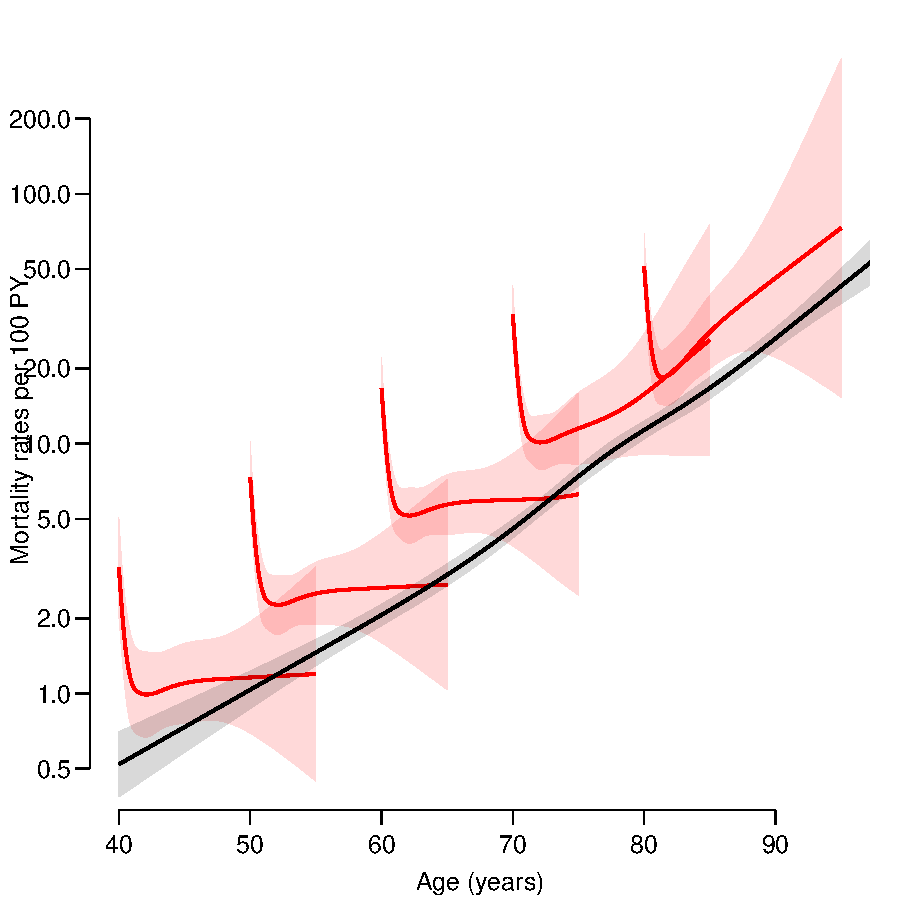
\includegraphics[width = 0.49\textwidth]{01flup-sep-mort}
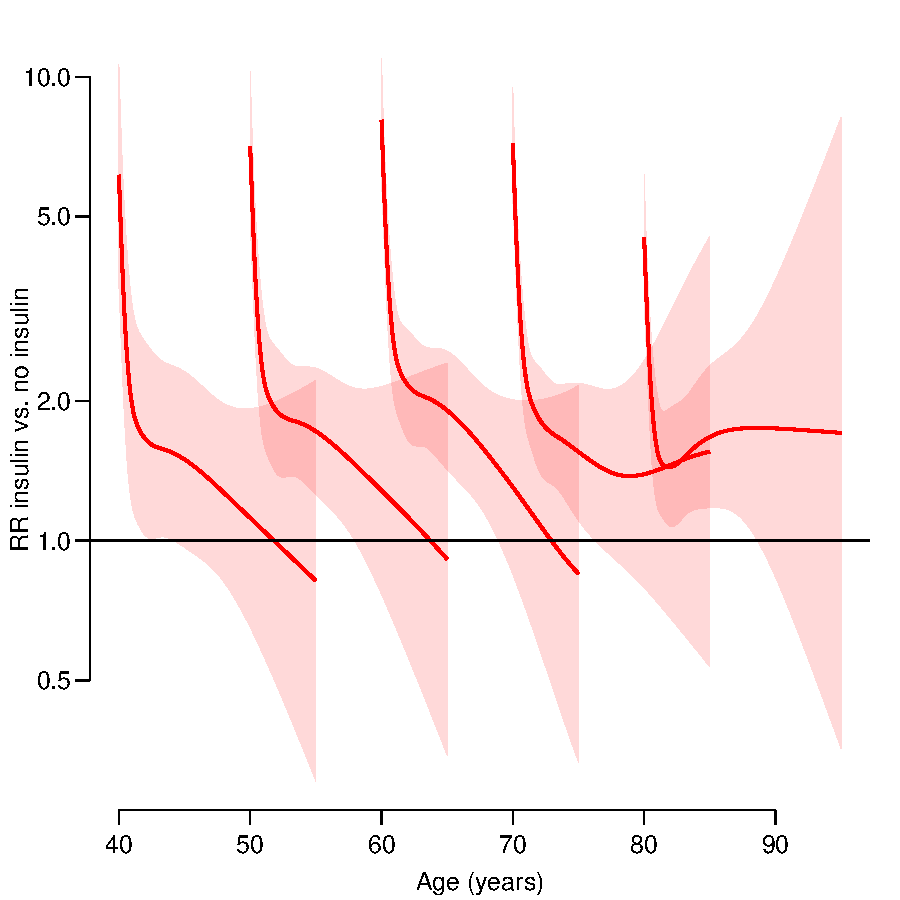
\includegraphics[width = 0.49\textwidth]{01flup-sep-HR}
\caption{\it Left panel: Mortality rates from separate models for the
  two mortality transitions; the \textrm{\tt
    DM}$\rightarrow$\textrm{\tt Dead} transition modeled by age alone;
  \textrm{\tt Ins}$\rightarrow$\textrm{\tt Dead} transition modeled
  with spline effects of current age, time since insulin and and age
  at insulin. \newline Right panel: Mortality HR of insulin vs. no insulin.}
\label{fig:Ins-noIns}
\end{figure}
The only difference between the interaction model and the two separate
models is that the latter allows different \texttt{sex}-effects
between mortality rates from \texttt{DM} and \texttt{Ins}. There
actually \emph{is} a difference between the estimates but hardly visible.

\chapter{More states}

\section{Subdividing states}

It may be of interest to subdivide the state \texttt{Dead} according
to whether the event has occurred or not. This will enable us to
estimate the number of patients that ever go on insulin.

This is done with \texttt{cutLexis} by using the argument
\texttt{split.states = TRUE}.
\begin{Schunk}
\begin{Sinput}
> dmCs <- cutLexis(data = dmS2,
+                   cut = dmS2$doins,
+             timescale = "per",
+             new.state = "Ins",
+             new.scale = "tfI",
+          split.states = TRUE)
> summary(dmCs)
\end{Sinput}
\begin{Soutput}
Transitions:
     To
From     DM  Ins Dead Dead(Ins)  Records:  Events: Risk time:  Persons:
  DM  35135 1694 2048         0     38877     3742   45885.49      9899
  Ins     0 5762    0       451      6213      451    8387.77      1791
  Sum 35135 7456 2048       451     45090     4193   54273.27      9996
\end{Soutput}
\end{Schunk}
We can illustrate the numbers and the transitions (figure
\ref{fig:box4}, p. \pageref{fig:box4})
\begin{Schunk}
\begin{Sinput}
> boxes(dmCs, boxpos = list(x = c(15, 15, 85, 85),
+                           y = c(85, 15, 85, 15)),
+       scale.R = 1000, show.BE = TRUE)
> legendbox(70, 50)
\end{Sinput}
\end{Schunk}
\insfig{box4}{0.7}{Transitions between 4 states: the numbers \emph{in}
  the boxes are person-years (middle), and below the number of persons
  who start, respectively end their follow-up in each of the states.}

Note that it is only the mortality rates that we have been modeling,
namely the transitions
\texttt{DM}$\rightarrow$\texttt{Dead} and
\texttt{Ins}$\rightarrow$\texttt{Dead(Ins)}.  If we were to model the
cumulative risk of using insulin or currently being on insulin we would
also need a model for the DM$\rightarrow$Ins transition. Subsequent to
that we would then compute the probability of being in each state
conditional on suitable starting conditions (including time of
start). With models where transition rates depend on several time
scales this is not a trivial task. This is treated in more detail in
the vignette on \texttt{simLexis}.

\section{Multiple intermediate events}

We may be interested in initiation of either insulin or OAD (oral
anti-diabetic drugs), thus giving rise to more states and more
time scales. This can be accomplished by the \texttt{mcutLexis}
function, that generalizes \texttt{cutLexis}:
\begin{Schunk}
\begin{Sinput}
> dmM <- mcutLexis(dmL,
+            timescale = "per",
+                   wh = c("doins", "dooad"),
+           new.states = c("Ins", "OAD"),
+           new.scales = c("tfI", "tfO"),
+         ties.resolve = TRUE)
\end{Sinput}
\begin{Soutput}
NOTE: Precursor states set to DM 
NOTE: 15 records with tied events times resolved (adding 0.01 random uniform),
      so results are only reproducible if the random number seed was set.
\end{Soutput}
\end{Schunk}
The \texttt{Lexis} machinery does not know what a reasonable order of
states is, so that will have to be fixed by hand using \texttt{Relevel}:
\begin{Schunk}
\begin{Sinput}
> levels(dmM)
\end{Sinput}
\begin{Soutput}
[1] "DM"      "Dead"    "OAD"     "Ins"     "OAD-Ins" "Ins-OAD"
\end{Soutput}
\begin{Sinput}
> dmM <- Relevel(dmM,  c("DM", "OAD", "Ins", "OAD-Ins", "Ins-OAD", "Dead"))
> summary(dmM, t = T)
\end{Sinput}
\begin{Soutput}
Transitions:
     To
From        DM  OAD  Ins OAD-Ins Ins-OAD Dead  Records:  Events: Risk time:  Persons:
  DM      2830 2958  688       0       0 1056      7532     4702   22920.14      7532
  OAD        0 3327    0    1006       0  992      5325     1998   22965.32      5325
  Ins        0    0  462       0     171  152       785      323    3883.13       785
  OAD-Ins    0    0    0     741       0  265      1006      265    3789.44      1006
  Ins-OAD    0    0    0       0     137   34       171       34     715.23       171
  Sum     2830 6285 1150    1747     308 2499     14819     7322   54273.27      9996

Timescales:
  per   age   tfD   tfI   tfO 
   ""    ""    "" "Ins" "OAD" 
\end{Soutput}
\end{Schunk}
We see that we now have two time scales defined as time since entry
into states.
\begin{Schunk}
\begin{Sinput}
> wh <- c(subset(dmM, lex.Cst == "Ins-OAD")$lex.id[1:2],
+         subset(dmM, lex.Cst == "OAD-Ins")$lex.id[1:2])
> print(subset(dmM, lex.id %in% wh), nd = 2)
\end{Sinput}
\begin{Soutput}
 lex.id     per   age  tfD  tfI  tfO lex.dur lex.Cst lex.Xst sex   dobth    dodm dodth
     18 1996.75 61.72 0.00   NA   NA    1.17      DM     OAD   M 1935.02 1996.75    NA
     18 1997.92 62.89 1.17   NA 0.00    8.08     OAD OAD-Ins   M 1935.02 1996.75    NA
     18 2005.99 70.97 9.25 0.00 8.08    4.00 OAD-Ins OAD-Ins   M 1935.02 1996.75    NA
     20 2009.25 53.22 0.00   NA   NA    0.03      DM     OAD   F 1956.03 2009.25    NA
     20 2009.27 53.25 0.03   NA 0.00    0.01     OAD OAD-Ins   F 1956.03 2009.25    NA
     20 2009.29 53.26 0.04 0.00 0.01    0.71 OAD-Ins OAD-Ins   F 1956.03 2009.25    NA
     38 2008.37 63.93 0.00   NA   NA    0.09      DM     Ins   M 1944.43 2008.37  2010
     38 2008.46 64.02 0.09 0.00   NA    0.21     Ins Ins-OAD   M 1944.43 2008.37  2010
     38 2008.67 64.24 0.31 0.21 0.00    1.33 Ins-OAD    Dead   M 1944.43 2008.37  2010
     39 2005.96 55.53 0.00   NA   NA    0.06      DM     Ins   M 1950.44 2005.96    NA
     39 2006.02 55.58 0.06 0.00   NA    0.03     Ins Ins-OAD   M 1950.44 2005.96    NA
     39 2006.05 55.61 0.09 0.03 0.00    3.95 Ins-OAD Ins-OAD   M 1950.44 2005.96    NA
   dooad   doins  dox
 1997.92 2005.99 2010
 1997.92 2005.99 2010
 1997.92 2005.99 2010
 2009.27 2009.29 2010
 2009.27 2009.29 2010
 2009.27 2009.29 2010
 2008.67 2008.46 2010
 2008.67 2008.46 2010
 2008.67 2008.46 2010
 2006.05 2006.02 2010
 2006.05 2006.02 2010
 2006.05 2006.02 2010
\end{Soutput}
\end{Schunk}
\begin{expl}
  We use subset to locate all records with \texttt{lex.Cst} equal to
  \texttt{Ins-OAD}, resp. \texttt{OAD-Ins}, and extract the ids
  (\texttt{lex.id}) from these. We the select the two first of each,
  and print all records for these persons.
\end{expl}
We can also illustrate the transitions to the different states, as in
figure \ref{fig:mbox} --- the specification of the \texttt{boxpos}
argument is facilitated by the logical ordering of the states
\begin{Schunk}
\begin{Sinput}
> boxes(dmM, boxpos = list(x = c(15, 40, 40, 85, 85, 80),
+                          y = c(50, 90, 10, 90, 10, 50)),
+            scale.R = 1000, show.BE = TRUE)
> legendbox(6, 95)
\end{Sinput}
\end{Schunk}
\insfig{mbox}{1.0}{Boxes for the \textrm{\tt dmM} object. The numbers
  \emph{in} the boxes are person-years (middle), and below the number
  of persons who start, respectively end their follow-up in each of
  the states.}
We may not be interested in whether persons were prescribed insulin
before OAD or vice versa, in which case we would combine the levels
with both insulin and OAD to one, regardless of order (figure
\ref{fig:mboxr}):
\begin{Schunk}
\begin{Sinput}
> summary(dmMr <- Relevel(dmM, list(1, 2, 3, 'OAD+Ins' = 4:5, 6)))
\end{Sinput}
\begin{Soutput}
Transitions:
     To
From        DM  OAD  Ins OAD+Ins Dead  Records:  Events: Risk time:  Persons:
  DM      2830 2958  688       0 1056      7532     4702   22920.14      7532
  OAD        0 3327    0    1006  992      5325     1998   22965.32      5325
  Ins        0    0  462     171  152       785      323    3883.13       785
  OAD+Ins    0    0    0     878  299      1177      299    4504.67      1177
  Sum     2830 6285 1150    2055 2499     14819     7322   54273.27      9996
\end{Soutput}
\begin{Sinput}
> boxes(dmMr, boxpos = list(x = c(15, 15, 85, 85, 50),
+                           y = c(85, 15, 85, 15, 50)),
+             scale.R = 1000, show.BE = TRUE)
\end{Sinput}
\end{Schunk}
\insfig{mboxr}{1.0}{Boxes for the \textrm{\tt dmMr} object with
  collapsed states. The numbers \emph{in} the boxes are person-years
  (middle), and below the number of persons who start, respectively
  end their follow-up in each of the states.}

Diagrams as those in figures
\ref{fig:mbox} and
\ref{fig:mboxr} gives an overview of the possible transitions,
which states it might be relevant to collapse, and which transitions
to model and how.

\subsection{Modeling rates}

The modeling of the transition rates is straightforward;
split the data along some timescale and then use \texttt{glmLexis} or
\texttt{gamLexis}, where it is possible to select the transitions
modeled. This is also possible with the \texttt{coxphLexis}
function, but it requires that a single time scale be selected as the
baseline time scale, and the effect of this will not be accessible.

Here is a brief sketch of models that might be considered:
\begin{Schunk}
\begin{Sinput}
> dmMs <- splitMulti(dmMr, age = 0:100)
> summary(dmMs)
\end{Sinput}
\begin{Soutput}
Transitions:
     To
From         DM   OAD  Ins OAD+Ins Dead  Records:  Events: Risk time:  Persons:
  DM      25682  2958  688       0 1055     30383     4701   22920.11      7532
  OAD         0 26226    0    1006  990     28222     1996   22959.19      5324
  Ins         0     0 4353     171  152      4676      323    3883.13       785
  OAD+Ins     0     0    0    5357  298      5655      298    4503.70      1177
  Sum     25682 29184 5041    6534 2495     68936     7318   54266.14      9995
\end{Soutput}
\begin{Sinput}
> levels(dmMs)
\end{Sinput}
\begin{Soutput}
[1] "DM"      "OAD"     "Ins"     "OAD+Ins" "Dead"   
\end{Soutput}
\begin{Sinput}
> rateIns <- gamLexis(dmMr, ~ s(age) + lex.Cst, from = 1:2   , to = 3:4)
\end{Sinput}
\begin{Soutput}
mgcv::gam Poisson analysis of Lexis object dmMr with log link:
Rates for transitions:
DM->Ins
OAD->OAD+Ins
\end{Soutput}
\begin{Sinput}
> rateOAD <- gamLexis(dmMr, ~ s(age) + lex.Cst, from = c(1,3), to = c(2, 4))
\end{Sinput}
\begin{Soutput}
mgcv::gam Poisson analysis of Lexis object dmMr with log link:
Rates for transitions:
DM->OAD
Ins->OAD+Ins
\end{Soutput}
\begin{Sinput}
> rateDth <- gamLexis(dmMr, ~ s(age) + lex.Cst)
\end{Sinput}
\begin{Soutput}
mgcv::gam Poisson analysis of Lexis object dmMr with log link:
Rates for transitions:
DM->Dead
OAD->Dead
Ins->Dead
OAD+Ins->Dead
\end{Soutput}
\begin{Sinput}
> ci.exp(rateIns, subset = "lex")
\end{Sinput}
\begin{Soutput}
           exp(Est.)     2.5%    97.5%
lex.CstOAD  1.867473 1.682872 2.072322
\end{Soutput}
\begin{Sinput}
> ci.exp(rateOAD, subset = "lex")
\end{Sinput}
\begin{Soutput}
           exp(Est.)      2.5%     97.5%
lex.CstIns 0.4964878 0.4237129 0.5817622
\end{Soutput}
\begin{Sinput}
> ci.exp(rateDth, subset = "lex")
\end{Sinput}
\begin{Soutput}
               exp(Est.)      2.5%    97.5%
lex.CstOAD     0.9461298 0.8675534 1.031823
lex.CstIns     2.6395092 2.2220452 3.135404
lex.CstOAD+Ins 1.6368495 1.4394540 1.861314
\end{Soutput}
\end{Schunk}

\chapter{\texttt{Lexis} functions}

\hypertarget{lexfun}{The \texttt{Lexis} machinery} has evolved over
  time since it was first introduced in a workable version in
  \texttt{Epi\_1.0.5} in August 2008.

  Over the years there have been additions of tools for handling
  multistate data. Here is a list of the current functions relating to
  \texttt{Lexis} objects with a very brief description; it does not
  replace the documentation, so read that before use. Unless otherwise
  stated, functions named \texttt{something.Lexis} (with a
  ``\texttt{.}'')  are S3 methods for \texttt{Lexis} objects, so you
  can skip the ``\texttt{.Lexis}'' in daily use.

\setlist{noitemsep}
\begin{description}

% \item[Define]\ \\
%   \begin{tabular}{rp{0.8\linewidth}}
%  \texttt{cal.yr} & transforms \texttt{Date} variables (measured in
%                    days) to \texttt{cal.yr} format (measured in
%                    years)\\
%   \texttt{Lexis} & defines a \texttt{Lexis} object\\
% \texttt{unLexis} & remove \texttt{Lexis} specific attributes\\
%   \end{tabular}

\item[Define]\ \\
\begin{description}
\item[\texttt{Lexis}] defines a \texttt{Lexis} object
\item[\texttt{cal.yr}] transforms \texttt{Date} variables (measured in
  days) to \texttt{cal.yr} format (measured in years)
\end{description}

\item[Cut and split]\ \\
\begin{description}
\item[\texttt{cutLexis}] cut follow-up at intermediate event
\item[\texttt{mcutLexis}] cut follow-up at multiple intermediate
  events, keeping track of history
\item[\texttt{rcutLexis}] cut follow-up at intermediate, possibly
  recurring, events, only recording the current state
\item[\texttt{countLexis}] cut follow-up at intermediate event time and count
  the no. events so far
\item[\texttt{splitLexis}] split follow up along a time scale
\item[\texttt{splitMulti}] split follow up along several time scales --- from
  the \texttt{popEpi} package, faster and has simpler syntax than
  \texttt{splitLexis}
\item[\texttt{addCov.Lexis}] add clinical measurements at a given date to a
  \texttt{Lexis} object
\item[\texttt{addDrug.Lexis}] add drug exposures to a \texttt{Lexis} object
\item[\texttt{coarse.Lexis}] combine successive records in a \texttt{Lexis} object
\end{description}

% \item[Boxes and plots]\ \\
% \begin{tabular}{rl}
% \texttt{boxes.Lexis} & draw a diagram of states and transitions\\
% \texttt{legendbox} & draw a box explaining the numbers output by \texttt{boxes.Lexis}\\
% \texttt{plot.Lexis} & draw a standard Lexis diagram\\
% \texttt{points.Lexis} & add points to a Lexis diagram\\
% \texttt{lines.Lexis} & add lines to a Lexis diagram\\
% \texttt{PY.ann.Lexis} & annotate life lines in a Lexis diagram
% \end{tabular}

\item[Boxes and plots]\ \\
\begin{description}
\item[\texttt{boxes.Lexis}] draw a diagram of states and transitions
\item[\texttt{legendbox}] draw a box explaining the numbers output by \texttt{boxes.Lexis}
\item[\texttt{plot.Lexis}] draw a standard Lexis diagram
\item[\texttt{points.Lexis}] add points to a Lexis diagram
\item[\texttt{lines.Lexis}] add lines to a Lexis diagram
\item[\texttt{PY.ann.Lexis}] annotate life lines in a Lexis diagram
\end{description}

\newpage
\item[Summarize and query]\ \\
\begin{description}
\item[\texttt{summary.Lexis}] overview of transitions, risk time etc.
\item[\texttt{levels.Lexis}] what are the states in the \texttt{Lexis} object
\item[\texttt{paths.Lexis}] what are the paths through states in a \texttt{Lexis} object
\item[\texttt{nid.Lexis}] number of persons in the \texttt{Lexis}
  object --- how many unique values of \texttt{lex.id} are present
\item[\texttt{entry}] entry time
\item[\texttt{exit}] exit time
\item[\texttt{status}] status at entry or exit
\item[\texttt{timeBand}] factor of time bands
\item[\texttt{timeScales}] what time scales are in the \texttt{Lexis} object
\item[\texttt{timeSince}] what time scales are defined as time since a given state
\item[\texttt{breaks}] what breaks are currently defined
\item[\texttt{absorbing}] what are the absorbing states
\item[\texttt{transient}] what are the transient states
\item[\texttt{preceding}, \texttt{before}] which states precede this
\item[\texttt{succeeding}, \texttt{after}] which states can follow this
\item[\texttt{tmat.Lexis}] transition matrix for the \texttt{Lexis} object
\end{description}

\item[Manipulate]\ \\
\begin{description}
\item[\texttt{subset.Lexis}, \texttt{[}] subset of a \texttt{Lexis} object
\item[\texttt{merge.Lexis}] merges a \texttt{Lexis} objects with a
  \texttt{data.frame}
\item[\texttt{cbind.Lexis}] bind a \texttt{data.frame} to a \texttt{Lexis} object
\item[\texttt{rbind.Lexis}] put two \texttt{Lexis} objects head-to-foot
\item[\texttt{order.Lexis}, \texttt{orderLexis}] ordering of records
  in a \texttt{Lexis} object
\item[\texttt{sortLexis}] sort records in a \texttt{Lexis} object by
  (\texttt{lex.id}, \texttt{time}) 
\item[\texttt{transform.Lexis}] transform and add variables
\item[\texttt{tsNA20}] turn \texttt{NA}s to 0s for time scales
\item[\texttt{factorize.Lexis}] turn \texttt{lex.Cst} and
  \texttt{lex.Xst} into factors with levels equal to the actually
  occurring values in both
\item[\texttt{Relevel.Lexis}] reorder and/or combine states
\item[\texttt{rm.tr}] remove transitions from a \texttt{Lexis} object
\item[\texttt{bootLexis}] bootstrap sample of \emph{persons}
  (\texttt{lex.id}) from a \texttt{Lexis} object
\item[\texttt{unLexis}] remove \texttt{Lexis} attributes from a
  \texttt{Lexis} object
\end{description}

\item[Simulate]\ \\
\begin{description}
\item[\texttt{simLexis}] simulate a \texttt{Lexis} object from
  specified transition rate models
\item[\texttt{nState}, \texttt{pState}] count state occupancy from a
  simulated \texttt{Lexis} object
\item[\texttt{plot.pState}, \texttt{lines.pState}] plot state occupancy from a
  \texttt{pState} object
\end{description}

\item[Stack]\ \\
\begin{description}
\item[\texttt{stack.Lexis}] make a stacked object for simultaneous
  analysis of transitions --- returns a \texttt{stacked.Lexis} object
\item[\texttt{subset.stacked.Lexis}] subsets of a \texttt{stacked.Lexis} object
\item[\texttt{transform.stacked.Lexis}] transform  a \texttt{stacked.Lexis} object
\end{description}

\newpage
\item[Interface to other packages]\ \\
\begin{description}
\item[\texttt{msdata.Lexis}] interface to \texttt{mstate} package
\item[\texttt{etm.Lexis}] interface to \texttt{etm} package
\item[\texttt{crr.Lexis}] interface to \texttt{cmprsk} package
\end{description}

\item[Statistical models]\ \\
\begin{description}
\item[\texttt{AaJ.Lexis}] compute the Aalen-Johansen estimator for a
  \texttt{Lexis} object --- wrapper for \texttt{survfit} from
  \texttt{survival}
\item[\texttt{ci.Crisk}] compute cumulative risks with CIs from model
  objects for competing rates
\item[\texttt{glmLexis}] fit a \texttt{glm} model using the
  \texttt{poisreg} family to (hopefully) time split data
\item[\texttt{gamLexis}] fit a \texttt{gam} model (from the
  \texttt{mgcv} package) using the \texttt{poisreg} family to
  (hopefully) time split data
\item[\texttt{coxphLexis}] fit a Cox model to follow-up in a
  \texttt{Lexis} object
\item In versions of Epi up to 2.56 the three modeling functions were called
  \texttt{glm.Lexis},
  \texttt{gam.Lexis} and
  \texttt{coxph.Lexis} --- but they are not S3 methods so the naming was
  illogical. The versions with the old names still exist in
  \texttt{Epi} for backward compatibility.
\end{description}
\end{description}
\begin{Schunk}
\begin{Soutput}
  Start time: 2025-10-06, 16:32:43 
    End time: 2025-10-06, 16:33:20 
Elapsed time: 0.62 minutes
\end{Soutput}
\end{Schunk}

\renewcommand{\bibname}{References}

\bibliographystyle{unsrt}%{plain}
\begin{thebibliography}{1}

\bibitem{Holford.1976}
T~R Holford.
\newblock Life tables with concomitant information.
\newblock {\em Biometrics}, 32:587--597, 1976.

\bibitem{Whitehead.1980}
J~Whitehead.
\newblock Fitting {C}ox's regression model to survival data using {GLIM}.
\newblock {\em Applied Statistics}, 29(3):268--275, 1980.

\bibitem{Plummer.2011}
M~Plummer and B~Carstensen.
\newblock Lexis: An {R} class for epidemiological studies with long-term
  follow-up.
\newblock {\em Journal of Statistical Software}, 38(5):1--12, 1 2011.

\bibitem{Carstensen.2011a}
B~Carstensen and M~Plummer.
\newblock Using {L}exis objects for multi-state models in {R}.
\newblock {\em Journal of Statistical Software}, 38(6):1--18, 1 2011.

\bibitem{Carstensen.2007a}
B~Carstensen.
\newblock Age-{P}eriod-{C}ohort models for the {L}exis diagram.
\newblock {\em Statistics in Medicine}, 26(15):3018--3045, July 2007.

\bibitem{Iacobelli.2013}
S~Iacobelli and B~Carstensen.
\newblock {Multiple time scales in multi-state models}.
\newblock {\em Stat Med}, 32(30):5315--5327, Dec 2013.

\end{thebibliography}

\addcontentsline{toc}{chapter}{\bibname}

\end{document}
